%%%%%%%%%%%%%%%%%%%%%%%%%%%%%%%%%%%%%%%%%%%%%%%%%%%%%%%%%%%%%%%%%%%%%%%%%%%%%%%%%%%%%%%%%%%
%%%% Die Dokumentenklasse und ihre Optionen %%%%%%%%%%%%%%%%%%%%%%%%%%%%%%%%%%%%%%%%%%%%%%%
\documentclass[captions=tableheading, 12pt, headings=small, parskip=half]{scrartcl}

%%%%%%%%%%%%%%%%%%%%%%%%%%%%%%%%%%%%%%%%%%%%%%%%%%%%%%%%%%%%%%%%%%%%%%%%%%%%%%%%%%%%%%%%%%%
%%%% LaTeX-Pakete %%%%%%%%%%%%%%%%%%%%%%%%%%%%%%%%%%%%%%%%%%%%%%%%%%%%%%%%%%%%%%%%%%%%%%%%%
\usepackage[utf8]{inputenc}
\usepackage[T1]{fontenc}
\usepackage[ngerman]{babel}
\usepackage{setspace,               % Zeilendurchschuss verändern (\doublespacing,\onehalfspacing)
            booktabs,               % Schöne Tabellen
            amsmath,                % Mathepackage der American Mathematical Society
            amsfonts,               % Paket für schönere mathematische Schriftarten
            amssymb,                % Paket für schönere mathematische Symbole
            bbm, 					% Blackboard-Style im Mathemodus
            bm, 					% Bold-Symbols im Mathemodus
            enumitem, 				% Anpassungen der enumerate-Umgebung
            graphicx,               % Paket zum Laden von Graphiken
            lmodern,                % Schrifttyp, der mit Microtype zusammenarbeitet
            nicefrac,				% Schräge Brüche
            csquotes,				% für Anführungszeichen
            microtype,              % Typographische Korrekturen bei Umbrüchen
            hyperref,				% url-Befehl
            calligra,
            setspace,
            multirow,
            empheq,
            xcolor,
            dsfont,
            nicefrac,
            float,
            mathtools,
            animate,
            blkarray
}


\usepackage[most]{tcolorbox}

\usepackage{tikz,tkz-tab}
\usepackage[left=2.5cm,right=2.5cm,top=2cm,bottom=2cm]{geometry} % Seiteneinrichtung
%\usepackage{geometry} % Seiteneinrichtung

\usepackage{dcolumn}
\newcolumntype{d}[1]{D{.}{.}{#1}}

\newcommand{\mybox}[2][blue!15]{%
	\vspace{-0.5cm}
	\begin{center}%
		\begin{tikzpicture}%
		\node[rectangle, draw=#1, top color=#1, bottom color=#1, 
		rounded corners=5pt, inner xsep=5pt, inner ysep=6pt, outer ysep=10pt]{
			\begin{minipage}{1.05\linewidth}#2\end{minipage}};%
		\end{tikzpicture}%
	\end{center}%
}

\newcolumntype{L}{>{$}l<{$}}
\newcolumntype{R}{>{$}r<{$}}
\newcolumntype{C}{>{$}c<{$}}



\begin{document}
\begin{table}[H]
\begin{tabular}{lr}
	& \multirow{4}{*}{\includegraphics[width = 8cm]{Code1/wwu_logo.png}}\\
	Dr. Willi Mutschler& \\
	M.Sc. Manuel Stapper & \\
	Winter term 2017/2018 \hphantom{MMMMMMMMMMM}& 
\end{tabular}
\end{table}
\vspace{1cm}
\begin{center}
{\Large Econometrics I} \\
-- Exercise Book --
\end{center}


\section*{\underline{Exercise 1}}
Let $A = [a_{ij}]\in\mathbb{R}^{n\times n}$ be a matrix and let $a = (a_1,...,a_n)'$, $x = (x_1,...,x_n)'$, $y = (y_1,...,y_n)'$ be vectors of length $n$.
\begin{enumerate}[label = \alph*)]
	\item Write the sum $\sum_{i=1}^n a_i\cdot x_i$ as a product of vectors.
	\mybox{$\sum_{i=1}^n a_i\cdot x_i = a'x$}
	\item Write $c_i = \sum_{j=1}^n a_{ij}\cdot x_j$ in matrix form.
	\mybox{$\sum_{j=1}^n a_{ij}\cdot x_j = A\cdot x$}
	\item Write $\sum_{i=1}^n y_i$ in matrix form. Hint: Use a vector of ones.
	\mybox{Let $\mathds{1}_n$ be a column vector of length $n$ containing only ones.\\
	$\sum_{i=1}^n y_i = \mathds{1}_n'\cdot y = y'\cdot\mathds{1}_n$}
	\item Write $\sum_{i=1}^n\sum_{j=1}^n a_{ij}$ in matrix form.
	\mybox{$\sum_{i=1}^n\sum_{j=1}^n a_{ij} = \mathds{1}_n'\cdot A \cdot \mathds{1}_n$}
\end{enumerate}



\section*{\underline{Exercise 2}}
Consider the following matrices
\[ A = \left(\begin{array}{d{2.0}d{2.0}d{2.0}}
1 & -1 & 2 \\
3 & 0 & 1 \\
2 & 1 & 0 \\
\end{array}\right),\qquad
B = \left(\begin{array}{c}
1 \\ 2 \\3\\ \end{array}\right),\qquad
C = \left(\begin{array}{d{2.0}d{2.0}d{2.0}}
2 & 0 & 3 \\
7 & -1 & 2 \\
0 & 1 & 1 \\
\end{array}\right)\]

\[ D = \left(\begin{array}{d{2.0}d{2.0}d{2.0}}
2 & 3  \\
-2 & 1 \\
0 & 5 \\
\end{array}\right),\qquad
E = \left(\begin{array}{ccc}
0 & 2 & 1\\
\end{array}\right).
\]
\begin{enumerate}[label = \alph*)]
	\item Calculate (if possible): $AB$, $CD$, $EA$, $BE$, $ED$.
	\mybox{
		\[
		AB = \left(\begin{array}{d{1.0}d{1.0}}
		5\\6\\4
		\end{array}\right),\qquad
		CD = \left(\begin{array}{d{2.0}d{2.0}}
		4&21\\16&30\\-2&6
		\end{array}\right)
		\qquad
		EA = \left(\begin{array}{d{1.0}d{1.0}d{1.0}}
		8&1&2
		\end{array}\right)
		\]
	}
	\mybox{
		\[
		BE = \left(\begin{array}{d{1.0}d{1.0}d{1.0}}
		0&2&1\\0&4&2\\0&6&3
		\end{array}\right),\qquad
		ED = \left(\begin{array}{d{2.0}d{2.0}}
		-4&7
		\end{array}\right)
		\]
	}
	\item Verify that: $(A+C)' = A' + C'$ and $(AC)'=C'A'$.
	\mybox{
		\begin{align*}
			(A+C)' &= \left[\left(\begin{array}{d{2.0}d{2.0}d{2.0}}
				1 & -1 & 2 \\ 3 & 0 & 1 \\ 2 & 1 & 0 \\
			\end{array}\right) + 
			\left(\begin{array}{d{2.0}d{2.0}d{2.0}}
				2 & 0 & 3 \\ 7 & -1 & 2 \\ 0 & 1 & 1 \\
			\end{array}\right)\right]'\\
			&= 	\left(\begin{array}{d{2.0}d{2.0}d{2.0}}
				3 & -1 & 5 \\ 10 & -1 & 3 \\ 2 & 2 & 1
			\end{array}\right)'\\
			&= \left(\begin{array}{d{2.0}d{2.0}d{2.0}}
				3 & 10 & 2 \\ -1 & -1 & 2 \\ 5 & 3 & 1 
			\end{array}\right)\\
			A' + C' &= 
			\left(\begin{array}{d{2.0}d{2.0}d{2.0}}
				1&3&2\\-1&0&1\\2&1&0
			\end{array}\right) + 
			\left(\begin{array}{d{2.0}d{2.0}d{2.0}}
				2&7&0\\0&-1&1\\3&2&1
			\end{array}\right)\\
			&= \left(\begin{array}{d{2.0}d{2.0}d{2.0}}
				3 & 10 & 2 \\ -1 & -1 & 2 \\ 5 & 3 & 1 
			\end{array}\right)
		\end{align*}
		
		\begin{align*}
			(AC)' &= \left[\left(\begin{array}{d{2.0}d{2.0}d{2.0}}
				1 & -1 & 2 \\ 3 & 0 & 1 \\ 2 & 1 & 0 \\
			\end{array}\right) \cdot 
			\left(\begin{array}{d{2.0}d{2.0}d{2.0}}
				2 & 0 & 3 \\ 7 & -1 & 2 \\ 0 & 1 & 1 \\
			\end{array}\right)\right]'\\
			&= \left(\begin{array}{d{2.0}d{2.0}d{2.0}}
				-5&6&11\\3&1&-1\\3&10&8
			\end{array}\right) = C'A'
		\end{align*}
	}
\end{enumerate}

\section*{\underline{Exercise 3}}

Consider the following matrices
\[ A= \left(\begin{array}{d{2.0}d{2.0}}
1 & -1 \\
2 & 1 \\
\end{array}\right),\qquad
B= \left(\begin{array}{d{2.0}d{2.0}}
0 & -2 \\
1 & -3 \\
\end{array}\right).\]
\begin{enumerate}[label = \alph*)]
	\item Calculate the determinant of $A$, $B$, $AB$, $A'$, $2A$ and $-B$.
	\mybox{
	\[
	\det(A) = 3, \qquad \det(B) = 2, \qquad \det(AB) = 6 = \det(A)\det(B),
	\]
	\[
	\det(A') = 3 = \det(A), \qquad \det(2A) = 12 = 2^2\det(A),
	\]
	\[
	\det(-B) = 2 = \det(B) = (-1)^2\det(B)
	\]
	}
	\item Calculate $A^{-1}$ and $B^{-1}$.
	\mybox{
		\[
		A^{-1} = \frac{1}{3}\cdot \left(\begin{array}{d{2.0}d{2.0}}
		1&1\\-2&1
		\end{array}\right)\text{ ,}
		\qquad
		B^{-1} = \frac{1}{2}\cdot \left(\begin{array}{d{2.0}d{2.0}}
		-3&2\\-1&0
		\end{array}\right)
		\]	
	}
	\item Calculate $(AB)^{-1}$.
	\mybox{
		\[
		(AB)^{-1} = -\frac{1}{6}\left(\begin{array}{d{2.0}d{2.0}}
		7&1\\1&1
		\end{array}\right)
		\]	
	}
	\item Calculate $B^{-1}A^{-1}$ and compare with (b).
	\mybox{
		\[
		B^{-1}A^{-1} = -\frac{1}{6}\left(\begin{array}{d{2.0}d{2.0}}
		7&1\\1&1
		\end{array}\right) = (AB)^{-1}
		\]	
	}
	\item Are the matrices $A$ and $C=A'A$ positive definite, negative definite or indefinite?
	\mybox{
		Approach 1:\\
		The matrix $A$ is positive definite, if $x'Ax>0$ for every vector $x\ne 0$,\\
		negative definite if $x'Ax>0$\\
		and indefinite, if there exist $x, y$ for which $x'Ax>0$ and $y'Ay<0$.\\
		\begin{align*}
			x'Ax &= \begin{pmatrix} x_1& x_2 \end{pmatrix}
			\left(\begin{array}{d{2.0}d{2.0}}1&-1\\2&1\end{array}\right)
			\begin{pmatrix} x_1\\ x_2 \end{pmatrix}\\
			&= x_1^2 + x_1x_2 + x_2^2
		\end{align*}
		Case 1: $x_1x_2 \ge 0$:  $x'Ax>0$\\
		Case 2: $x_1x_2 < 0$:\\
		$x'Ax = x_1^2 + x_1x_2 + x_2^2 > x_1^2 + 2x_1x_2 + x_2^2 = (x_1 + x_2)^2 > 0$\\
		$\Rightarrow$ $x'Ax > 0$ for every vector $x\ne 0$ $\Rightarrow$ $A$ is positive definite.
	}
	
	\mybox{
		Approach 2:\\
		A matrix $A$ is positive definite if every principle minor is positive,\\
		negative definite if odd principle minors are negative and even principle minors are positive\\
		and indefinite if the determinant is not zero and the matrix is neither p.d. nor n.d.\\
		For a matrix
		\[
			C = \begin{pmatrix}a&b\\c&d\end{pmatrix}
		\]the first principle minor is $a$ and the second $\det(C)=ad - bc$.\\
		The first principle minor of $A$ is 1 and the second principle minor is 3, so $A$ is positive definite.
	}
	
	\mybox{
		$A'A$ is a so-called quadratic form and thus positive definite. This can be seen as follows:
		\[
		x'A'Ax = (x'A')(Ax) = (Ax)'\underbrace{Ax}_{=: y} = y'y = y_1^2 + y_2^2 + ... + y_n^2 \ge 0
		\]Both of the above approaches would of course give the same result.
	}
	\item Give an example of a negative definite and indefinite (2 $\times$ 2) matrix.
	\mybox{
		Since $A$ is positive definite, $(-1)\cdot A$ is negative definite:\\
		$x'Ax > 0$ $\Leftrightarrow$ $(-1)\cdot x'Ax = x'(-1)\cdot Ax < 0$\\
		The matrix $D = \left(\begin{array}{d{2.0}d{2.0}}1&0\\0&-1\end{array}\right)$ is indefinite, because there are two vectors $x = \begin{pmatrix}1&0\end{pmatrix}'$ and $y = \begin{pmatrix}0&1\end{pmatrix}'$ so that $x'Dx = 1 > 0$ and $y'Dy = -1 < 0$.
	}
\end{enumerate}

\section*{\underline{Exercise 4}}
In this exercise we take a look at an example to understand why the unbiased variance estimator has a factor $\frac{1}{T-1}$ instead of $\frac{1}{T}$. Imagine a box containing 3 coins with values 0, 2 and 4 denoted as $x_1, x_2$ and $x_3$ respectively. Please follow the steps:
\begin{itemize}
	\item Calculate the \textit{population sample} \[\mu := \frac{x_1 + x_2 + x_3}{3}\] and the \textit{population variance} \[\sigma^2 = \frac{1}{3}\sum_{t = 1}^3{(x_i - \mu)^2}\text{ .}\]
	\item We try to estimate the population variance by drawing a coin $T = 2$ times. Write down every combination of two values from the population. Hint: $(0, 2)\ne (2, 0)$
	\item For every of these 9 combinations, calculate the sample average and the sample variance with both factors $\frac{1}{T}$ and $\frac{1}{T-1}$.
	\item Calculate the average of these three key figures over all 9 samples.
	\item What do you notice?
\end{itemize}
\mybox{
	\begin{table}[H]
		\centering
		\begin{tabular}{cccc}
			\toprule
			\toprule
			Sample & Sample Mean & Sample variance $\left(\nicefrac{1}{T}\right)$& Sample variance $\left(\nicefrac{1}{T-1}\right)$\\
			\midrule
			(0,0)&0&0&0\\
			(0,2)&1&1&2\\
			(0,4)&2&4&8\\
			(2,0)&1&1&2\\
			(2,2)&2&0&0\\
			(2,4)&3&1&2\\
			(4,0)&2&4&8\\
			(4,2)&3&1&2\\
			(4,4)&4&0&0\\
			\midrule
			Average&2&$\nicefrac{4}{3}$&$\nicefrac{8}{3}$\\
			\bottomrule
			\bottomrule
		\end{tabular}
	\end{table}

}

\section*{\underline{Exercise 5}}

An investor wants to invest in two possible, independent stocks $A$ and $B$. The return of those two stocks is denoted as $R_A$ and $R_B$. To evaluate the stocks we assume
\[
\operatorname{E}(R_A) = 2 \qquad \operatorname{E}(R_B) = 5 \qquad \operatorname{Var}(R_A) = 2 \qquad \operatorname{Var}(R_B) = 6
\]
\begin{enumerate}[label = \alph*)]
	\item Calculate the expected return in case the investor splits his capital evenly.
	\mybox{
		Let $p$ denote the proportion of capital invested in $B$. The return on the portfolio is then expressed as $(1-p)\cdot R_A + p\cdot R_B$.
	\[
	\operatorname{E}\left[(1-p)\cdot R_A + p\cdot R_B\right] = (1-p)\cdot\operatorname{E}(R_A) + p\cdot \operatorname{E}(R_B)
	\]
	For $p = \frac{1}{2}$ it yields $\frac{1}{2}\cdot 2 + \frac{1}{2}\cdot 5 = 3.5$
	}
	\item Calculate the variance of the above described portfolio. What do you notice?
	\mybox{
		\[
		\operatorname{Var}\left[(1-p)\cdot R_A + p\cdot R_B \right] = (1-p)^2\cdot\operatorname{Var}(R_A) + p^2\cdot\operatorname{Var}(R_B)
		\]
		And for $p=\frac{1}{2}$: $\frac{1}{4}\cdot 2 + \frac{1}{4}\cdot 6 = 2$
	}
	\item The investor wants to limit his risk, so that the variance in the portfolio return does not exceed 3.5. What is the maximal return on such a portfolio? How much so you suggest him to invest in $A$ and in $B$?
	\mybox{
	Using the above formula for the portfolio variance:
	\begin{align*}
		(1-p)^2\cdot\operatorname{Var}(R_A) + p^2\cdot\operatorname{Var}(R_B) &= (1-p)^2\cdot 2 + p^2\cdot 6\\
		&= 8 p^2 - 4p + 2
	\end{align*}
Solving $8 p^2 - 4p + 2 = 3.5$ for $p$ yields $p = \frac{3}{4}$.
	}
\end{enumerate}

\section*{\underline{Exercise 6}}
Let $a$ be a column vector of length $n$ and $A$ an ($n\times n$) matrix. For a scalar valued function $f(x)$ of a vector $x$,
\[ \frac{\partial f(x)}{\partial x} = \left[
\begin{array}{c} 
\partial f/\partial x_1\\
\vdots\\
\partial f/\partial x_n\\
\end{array} \right] \]
is called the gradient vector of $f$. For the vector $y = Ax$, define
\[
\frac{\partial y}{\partial x} = \begin{bmatrix}
\partial y_1/\partial x'\\
\partial y_2/\partial x'\\
\vdots\\
\partial y_n/\partial x'
\end{bmatrix}\text{ .}
\]

\begin{enumerate}[label = \alph*)]
	\item Show the following equations:
	\begin{enumerate}[label = \roman*)]
		\item $\frac{\partial a'x}{\partial x} = a$
		\mybox{
			\begin{align*}
				\frac{\partial a'x}{\partial x} &= 	\frac{\partial}{\partial x}\sum_{i=1}^n{a_ix_i}\\
				&= \left[\begin{array}{c}
					\frac{\partial}{\partial x_1} \sum_{i=1}^n{a_ix_i}\\
					\vdots\\
					\frac{\partial}{\partial x_n} \sum_{i=1}^n{a_ix_i}\\
				\end{array}\right]\\
				&= \left[\begin{array}{c}a_1\\\vdots\\a_n\end{array}\right] = a
			\end{align*}
		}
		\item $\frac{\partial Ax}{\partial x} = A$
		\mybox{
			\begin{align*}
				\frac{\partial Ax}{\partial x} &= \left[\begin{array}{c}
					\frac{\partial}{\partial x'}A_{1\bullet}x\\
					\vdots\\
					\frac{\partial}{\partial x'}A_{n\bullet}x
				\end{array}\right]\\
				&\overset{i)}{=} \left[\begin{array}{c} A_{1\bullet}\\\vdots\\A_{n\bullet}\end{array}\right]  = A
			\end{align*}
		}
		\newpage
		\item $\frac{\partial x'Ax}{\partial x} = (A + A')x$
		\mybox{
			\begin{align*}
				\frac{\partial x'Ax}{\partial x} &= \frac{\partial}{\partial x}\sum_{i=1}^n{\sum_{j = 1}^n{ a_{ij}x_ix_j }}\\
				&= \left[\begin{array}{c}
					\frac{\partial}{\partial x_1}\sum_{i=1}^n{\sum_{j = 1}^n{ a_{ij}x_ix_j }}\\
					\vdots\\
					\frac{\partial}{\partial x_n}\sum_{i=1}^n{\sum_{j = 1}^n{ a_{ij}x_ix_j }}
				\end{array}\right]\\
				&= \left[\begin{array}{c}
					\left(\sum_{i = 2}^n{a_{1i}x_i}\right) + 2a_{11}x_1 + \left(\sum_{i = 2}^n{a_{i1}x_i}\right)\\
					\vdots\\
					\left(\sum_{i = 2}^n{a_{ni}x_i}\right) + 2a_{nn}x_1 + \left(\sum_{i = 2}^n{a_{in}x_i}\right)
				\end{array}\right]\\
				&= \left[\begin{array}{c}
					\left(\sum_{i = 1}^n{a_{1i}x_i}\right) + \left(\sum_{i = 1}^n{a_{i1}x_i}\right)\\
					\vdots\\
					\left(\sum_{i = 1}^n{a_{ni}x_i}\right)  + \left(\sum_{i = 1}^n{a_{in}x_i}\right)
				\end{array}\right]\\
				&= Ax + A'x = (A + A')x
			\end{align*}
		}
	\end{enumerate}
	\item What does a) iii) imply for $\frac{\partial x'Ax}{\partial x}$ if $A$ is symmetric?
	\mybox{If $A$ is symmetric ($A'=A$), then $\frac{\partial x'Ax}{\partial x} = 2Ax$}
\end{enumerate}

\section*{\underline{Exercise 7}}

Consider the following linear regression:
\[
y_t = \alpha + \beta x_t + u_t\text{ ,}\qquad\text{ for }t=1,...,T\text{ .}
\]Show that the OLS estimators $\hat{\alpha}$ and $\hat{\beta}$ are given by
\[
\hat{\beta} = \frac{\sum_{t = 1}^T{(x_t - \bar{x})(y_t - \bar{y})}}{\sum_{t = 1}^T{(x_t - \bar{x})^2}}\text{ ,}\qquad \hat{\alpha} = \bar{y} - \hat{\beta}\bar{x}
\]
\mybox{
	Minimize $\sum_{t = 1}^T{\left[y_t - (\alpha + \beta x_t)\right]^2}$. Therefore derive w.r.t. $\alpha$ and $\beta$.
	\begin{alignat*}{2}
		\qquad&&  \frac{\partial}{\partial \alpha}\sum_{t = 1}^T{\left(y_t - \alpha - \beta x_t\right)^2} &\overset{!}{=} 0\\
		\Leftrightarrow\qquad&& \sum_{t = 1}^T{2\cdot(y_t - \alpha - \beta x_t)\cdot (-1)} &= 0\\
		\Leftrightarrow\qquad&& \sum_{t = 1}^T{(y_t - \alpha - \beta x_t)} &= 0\\
		\Leftrightarrow\qquad&& \sum_{t = 1}^T{y_t} - \sum_{t = 1}^T{\beta x_t} &= \sum_{t = 1}^T{\alpha}\\
		\Leftrightarrow\qquad&& \sum_{t = 1}^T{y_t} - \beta\sum_{t = 1}^T{x_t} &= T\alpha\\
		\Leftrightarrow\qquad&& \bar{y} - \beta\bar{x} &= \alpha\qquad(\star)\\
	\end{alignat*}
	
	\begin{alignat*}{2}
		\qquad&&  \frac{\partial}{\partial \beta}\sum_{t = 1}^T{\left(y_t - \alpha - \beta x_t\right)^2} &\overset{!}{=} 0\\
		\Leftrightarrow\qquad&& \sum_{t = 1}^T{2\cdot(y_t - \alpha - \beta x_t)\cdot(-x_t)} &= 0\\
		\Leftrightarrow\qquad&& \sum_{t = 1}^T{(y_t - \alpha - \beta x_t)\cdot x_t} &= 0\\
		\Leftrightarrow\qquad&& \sum_{t = 1}^T{y_tx_t} - \alpha\cdot\sum_{t = 1}^T{x_t} &= \beta \cdot \sum_{t = 1}^T{x_t^2}\\
		\overset{(\star)}{\Leftrightarrow}\qquad&& \sum_{t = 1}^T{y_tx_t} - (\bar{y} - \beta\bar{x})\cdot\sum_{t = 1}^T{x_t} &= \beta \cdot \sum_{t = 1}^T{x_t^2}\\
		\vdots\qquad&&&\\
		\Leftrightarrow\qquad&& \frac{\left(\sum_{t = 1}^T{y_tx_t}\right) - T\bar{y}\bar{x}}{\left(\sum_{t = 1}^T{x_t^2}\right) - T(\bar{x})^2} &= \beta\\
		\Leftrightarrow\qquad&& \frac{\sum_{t = 1}^T{(x_t - \bar{x})(y_t - \bar{y})}}{\sum_{t = 1}^T{(x_t - \bar{x})^2}} &= \beta
	\end{alignat*}
}

\section*{\underline{Exercise 8}}

A supermarket chain plans to investigate the connection between marketing expenditure for a certain product and the number of items sold. $T=10$ different but comparable markets are included in the study. For market $t$, marketing expenditure (in USD) and number of items sold are denoted as $x_t$ and $y_t$ respectively.\\
From this study, the following values are calculated:\\
\begin{align*}
&\bar{x}=1170 \qquad \sqrt{\frac{1}{10}\sum_{t = 1}^{10}{(x_t - \bar{x})^2}} = 415\\
&\sum_{t = 1}^{10}{y_t} = 3500 \qquad \sum_{t = 1}^{10}{y_t^2} = 1'300'000 \qquad \sum_{t = 1}^{10}{x_ty_t} = 4'443'000
\end{align*}
\begin{enumerate}[label = \alph*)]
	\item Calculate the OLS-estimates $\hat{\alpha}$ and $\hat{\beta}$ of the regression model\\
	$y_t = \alpha + \beta x_t + u_t$.
	\mybox{
		\begin{align*}
			\hat{\beta} &= \frac{\sum_{t = 1}^T{(x_t - \bar{x})(y_t - \bar{y})}}{\sum_{t = 1}^T{(x_t - \bar{x})^2}} = \frac{\left(\sum_{t = 1}^T{y_tx_t}\right) - T\bar{x}\bar{y}}{\sum_{t = 1}^T{(x_t - \bar{x})^2}}\\
			&= \frac{\left(\frac{1}{T}\cdot\sum_{t = 1}^T{y_tx_t}\right) - \bar{x}\bar{y}}{\frac{1}{T}\sum_{t = 1}^T{(x_t - \bar{x})^2}} = \frac{\frac{1}{10}\cdot 4443000 - 1170 \cdot 350}{415^2} \approx 0.202\\
			\hat{\alpha} &= \bar{y} - \hat{\beta}\bar{x} \approx 350 - 0.202\cdot 1170 = 113.66
		\end{align*}
	}
	\item How is $\beta$ interpreted from an economic point of view?
	\mybox{
		The assumed model and the estimate $\hat{\beta} = 0.202$ suggest that every dollar spent on marketing increases the number of articles sold by 0.202.
	}
	\item The manager of a market not included in the study wants to sell 500 products, what would you suggest him to spend on marketing according to the estimated regression?
	\mybox{
		We calculate the marketing expenditure $x$ using the formula $\hat{y} = \hat{\alpha} + \hat{\beta}\cdot x$ with a desired $\hat{y} = 500$ and obtain $x = \frac{500 - \hat{\alpha}}{\hat{\beta}} \approx 1912.35$
	}
	\item Calculate the coefficient of determination and interpret it.
	\mybox{
		The coefficient of determination can be expressed as squared correlation between $x$ and $y$.\\
		\begin{align*}
			\text{Cor}(x,y) &= \frac{\frac{1}{10}\sum_{t = 1}^{10}{(x_t - \bar{x})(y_t - \bar{y})}}{\sqrt{\frac{1}{10}\sum_{t = 1}^{10}{(x_t - \bar{x})^2}} \cdot \sqrt{\frac{1}{10}\sum_{t = 1}^{10}{(y_t - \bar{y})^2}}}\\
			&\hdots\\
			&= 0.96828\\
			R^2 &= 0.96828^2 \approx 0.9375
		\end{align*}
		The coefficient of determination is close to 1, indicating that a linear dependence between marketing expenditures and number of items sold is plausible.
	}
\end{enumerate}

\section*{\underline{Exercise 9}}
\begin{enumerate}[label = \alph*)]
	\item State the A-, B- and C-assumptions in your own words.\\
	\mybox{
		\begin{itemize}
			\item \textbf{A1}: There is no relevant variable left out in the regression and every variable included is relevant.
			\item \textbf{A2}: There is a linear dependency between $x_t$ and $y_t$.
			\item \textbf{A3}: The parameters are constant for each pair of observations.
			\item \textbf{B1}: E$(u_t)=0$. The deviations from observation $y_t$ and fitted value $\hat{y}_t = \hat{\alpha} + \hat{\beta}x_t$ spreads around zero.
			\item \textbf{B2}: The deviation $u_t = y_t - \hat{y}_t$ spreads evenly.
			\item \textbf{B3}: There is no dependency between the deviations $u_1,...,u_T$: Knowledge about $u_t$ does not give any information about $u_s$ ($t\ne s$).
			\item \textbf{B4}: The distribution of deviations $u_t$ is normal.
			\item \textbf{C1}: The exogenous variables $x_t$ can be controlled, they are not random.
			\item \textbf{C2}: The values of $x_t$ are not the same for every pair of observations.
		\end{itemize}
	}
	\item Give a counterexample of each assumption by drawing a picture if points $(x_t, y_t)$, if possible. Otherwise describe the counterexample in your own words.\\
	\mybox{
		Below plots display counterexamples to A-, B- and C-assumptions. The observations (points) are drawn together with the regression line (red, dashed) on the left hand side. Residuals are drawn on the right hand side. C1 is the only assumption for which a counterexample could not be drawn. Examples for exogenous variables, which can not be controlled are easily found.\\
		\begin{minipage}{0.05\columnwidth}
		\begin{center}
			\Large \textbf{A1}
		\end{center}
		\end{minipage}
		\hfill
		\begin{minipage}{0.46\columnwidth}
			\includegraphics[width= \columnwidth]{Code1/A1.jpeg}
		\end{minipage}
		\hfill
		\begin{minipage}{0.46\columnwidth}
			\includegraphics[width= \columnwidth]{Code1/A1_res.jpeg}
		\end{minipage}
	
		\begin{minipage}{0.05\columnwidth}
		\begin{center}
			\Large \textbf{A2}
		\end{center}
		\end{minipage}
		\hfill
		\begin{minipage}{0.46\columnwidth}
			\includegraphics[width= \columnwidth]{Code1/A2.jpeg}
		\end{minipage}
		\hfill
		\begin{minipage}{0.46\columnwidth}
			\includegraphics[width= \columnwidth]{Code1/A2_res.jpeg}
		\end{minipage}
	
		\begin{minipage}{0.05\columnwidth}
		\begin{center}
			\Large \textbf{A3}
		\end{center}
		\end{minipage}
		\hfill
		\begin{minipage}{0.46\columnwidth}
			\includegraphics[width= \columnwidth]{Code1/A3.jpeg}
		\end{minipage}
		\hfill
		\begin{minipage}{0.46\columnwidth}
			\includegraphics[width= \columnwidth]{Code1/A3_res.jpeg}
		\end{minipage}
	}

	\mybox{
		\begin{minipage}{0.05\columnwidth}
		\begin{center}
			\Large \textbf{B1}
		\end{center}
		\end{minipage}
		\hfill
		\begin{minipage}{0.46\columnwidth}
			\includegraphics[width= \columnwidth]{Code1/B1.jpeg}
		\end{minipage}
		\hfill
		\begin{minipage}{0.46\columnwidth}
			\includegraphics[width= \columnwidth]{Code1/B1_res.jpeg}
		\end{minipage}
	
		\begin{minipage}{0.05\columnwidth}
		\begin{center}
			\Large \textbf{B2}
		\end{center}
		\end{minipage}
		\hfill
		\begin{minipage}{0.46\columnwidth}
			\includegraphics[width= \columnwidth]{Code1/B2.jpeg}
		\end{minipage}
		\hfill
		\begin{minipage}{0.46\columnwidth}
			\includegraphics[width= \columnwidth]{Code1/B2_res.jpeg}
		\end{minipage}

		\begin{minipage}{0.05\columnwidth}
		\begin{center}
			\Large \textbf{B3}
		\end{center}
		\end{minipage}
		\hfill
		\begin{minipage}{0.46\columnwidth}
			\includegraphics[width= \columnwidth]{Code1/B3.jpeg}
		\end{minipage}
		\hfill
		\begin{minipage}{0.46\columnwidth}
			\includegraphics[width= \columnwidth]{Code1/B3_res.jpeg}
		\end{minipage}
	}
\mybox{
	The assumption C2 is needed to ensure for example the uniqueness of the OLS estimate. 
		\begin{minipage}{0.05\columnwidth}
		\begin{center}
			\Large \textbf{C2}
		\end{center}
		\end{minipage}
		\hfill
		\begin{minipage}{0.46\columnwidth}
			\includegraphics[width= \columnwidth]{Code1/C2_plot.jpeg}
		\end{minipage}
		\hfill
		\begin{minipage}{0.46\columnwidth}
			\includegraphics[width= \columnwidth]{Code1/C2.jpeg}
		\end{minipage}
}
\end{enumerate}
\section*{\underline{Exercise 10}}
Take a look at the 6 scatterplots below.
\begin{figure}[H]
	\begin{minipage}{0.32 \columnwidth}
		\includegraphics[width = \columnwidth]{Code1/plot1.png}
		\includegraphics[width = \columnwidth]{Code1/plot4.png}
	\end{minipage}
	\hfill
	\begin{minipage}{0.32 \columnwidth}
		\includegraphics[width = \columnwidth]{Code1/plot2.png}
		\includegraphics[width = \columnwidth]{Code1/plot5.png}
	\end{minipage}
	\hfill
	\begin{minipage}{0.32 \columnwidth}
		\includegraphics[width = \columnwidth]{Code1/plot3.png}
		\includegraphics[width = \columnwidth]{Code1/plot6.png}
	\end{minipage}
\end{figure}
\begin{enumerate}[label = \alph*)]
	\item Which of the A-, B- and C-assumptions are not satisfied in the individual cases?
	\mybox{
	\begin{figure}[H]
		\begin{minipage}{0.32\columnwidth}
			A1 - $x$ not relevant
		\end{minipage}
		\hfill
		\begin{minipage}{0.32\columnwidth}
			A2 - Not linear\\
			A3 - Structural break\\
			B3 - Maybe autocorrelation
		\end{minipage}
		\hfill
		\begin{minipage}{0.32\columnwidth}
			B2 - Heteroscedasticity
		\end{minipage}
	\end{figure}

	\begin{figure}[H]
	\begin{minipage}{0.32\columnwidth}
		A2 - Not linear\\
		B3 - Positive autocorrelation
	\end{minipage}
	\hfill
	\begin{minipage}{0.32\columnwidth}
		B3 - Neg. autocorrelation\\
		OR\\
		A3 - Structural break
	\end{minipage}
	\hfill
	\begin{minipage}{0.32\columnwidth}
		A3 - Structural break
	\end{minipage}
	\end{figure}
	}
	\item Which of the assumptions could be violated without being visible in a scatterplot?\\
	\mybox{
		\begin{itemize}
			\item Stochastic exogenous variables
			\item Measurement errors and thus E$(u_t) = 0$
			\item Relevant variables, that are left out? Workaround: Plot the residuals of models with and without the variable. If including the variable lowers the residuals significantly, it is probably relevant.
		\end{itemize}
	}
\end{enumerate}

\section*{\underline{Exercise 11}}
The figure below shows the fitted values of two different regressions $y_t = \alpha + \beta x_t + u_t$. Besides the OLS regression line, the Least Absolute Deviation (LAD) regression line is shown. The LAD-estimators $\tilde{\alpha}$ and $\tilde{\beta}$ are calculated by minimizing
\[
\sum_{t = 1}^{15}{|y_t - (\alpha + \beta x_t)|}\text{ .}
\]
\begin{figure}[h!]
	\begin{minipage}{0.49\columnwidth}
		\includegraphics[width = \columnwidth]{Code1/LADreg.jpeg}
	\end{minipage}
	\hfill
	\begin{minipage}{0.49\columnwidth}
		\begin{align*}
		\sum_{t = 1}^{15}{y_t} = 50.67 \quad \sum_{t = 1}^{15}{y_t^2} = 219.53\\
		\sum_{t = 1}^{15}{\hat{y}_t^2} = 188.77 \quad \sum_{t = 1}^{15}{\tilde{y}_t} = 44.16\\
		\sum_{t = 1}^{15}{\tilde{y}_t^2} = 148.48
		\end{align*}
	\end{minipage}
\end{figure}
\begin{enumerate}[label = \alph*)]
	\item Calculate the coefficient of determination $R^2$ for both regressions using the above sums.
	\mybox{
	\begin{align*}
		R^2_{\text{OLS}} &= \frac{\sum_{t = 1}^T{(\hat{y}_t - \bar{y})^2}}{\sum_{t = 1}^T{(y_t - \bar{y})^2}}\\
		&= \frac{\left(\sum_{t = 1}^T{\hat{y}_t^2}\right) - T\bar{y}^2}{ \left( \sum_{t = 1}^T{y_t^2}\right) - T\bar{y}^2}\\
		&= \frac{188.77 - 15\cdot \left(\frac{50.67}{15}\right)^2}{219.53 - 15\cdot \left(\frac{50.67}{15}\right)^2}\approx 0.3640\\
		R^2_{\text{LAD}} &=  \frac{\sum_{t = 1}^T{(\tilde{y}_t - \bar{y})^2}}{\sum_{t = 1}^T{(y_t - \bar{y})^2}}\\
		&= \frac{\left(\sum_{t = 1}^T{\tilde{y}_t^2}\right) - 2\bar{y}\left(\sum_{t = 1}^T{\tilde{y}_t}\right) + N\bar{y}^2}{ \left( \sum_{t = 1}^T{y_t^2}\right) - T\bar{y}^2}\\
		&= \frac{148.48 - 2\cdot \frac{50.67}{15}\cdot 44.16 + 15\cdot \left(\frac{50.67}{15}\right)^2}{219.53 - 15\cdot \left(\frac{50.67}{15}\right)^2}\approx 0.4403
	\end{align*}

	}
	\item Calculate the correlation between $y_t$ and $x_t$.\mybox{
	\[\text{Cor}(x,y) = \sqrt{R^2_{\text{OLS}}}\cdot \text{sign}(\hat{\beta}) = \sqrt{0.3640} = 0.6033  \]
	}
	\item Interpret the above results.
	\mybox{
		The $R^2$ from LAD estimation is higher than the $R^2$ from OLS. The LAD-regression line suits the data better than the OLS-regression line. The reason for it is the outlier, which has a higher impact on the OLS estimation. LAD estimation is influences less and is called more robust against outliers.
	}
\end{enumerate}

\section*{\underline{Exercise 12}}
\begin{enumerate}[label = \alph*)]
	\item Consider the regression model \[y_t = \alpha + \beta x_t + u_t\text{ .}\]Is it possible that the coefficient of determination is either negative or larger than 1? Justify your answer briefly.
	\mybox{
		The $R^2$ in this case is the squared correlation. Since the correlation only takes values between -1 and 1, it holds that $0\le R^2 \le 1$.
	}
	\item Consider the regression model \[y_t = \alpha x_t + u_t\text{ .}\]Is it possible that the coefficient of determination is negative or larger than 1? Justify your answer.
	\mybox{
		$R^2$ is never larger than 1, because $R^2>1$ would imply
		\[
			\frac{\sum_{t = 1}^T{(y_t - \hat{y}_t)^2}}{\sum_{t = 1}^T{(y_t - \bar{y}_t)^2}} < 0\text{ .}
		\]Both sums are positive and therefore it holds that $R^2\le 1$.\\
		It can be negative in this case due to the fast that the regression line is forced to go through the origin. A proof is left out.
	}
\end{enumerate}


\section*{\underline{Exercise 13}}
Consider the following regression:
\[
	y_t = \alpha x_t + u_t\text{, \qquad where } u_t\sim \mathcal{N}(0, \sigma^2)
\]for $t = 1,...,T$. Assume validity if all A-, B- and C- assumptions.
\begin{enumerate}[label = \alph*)]
	\item Verify that the OLS estimator $\hat{\alpha}$ satisfies the following relationships
	\[
		\hat{\alpha} = \frac{\sum_{t = 1}^T{x_ty_t}}{\sum_{t = 1}^T{x_t^2}}
	\]and can be represented as
	\[
		\hat{\alpha} = \alpha + \frac{\sum_{t = 1}^T{x_tu_t}}{\sum_{t = 1}^T{x_t^2}} \text{ .}
	\]
	\mybox{
		\begin{align*}
			\hat{\alpha} &= \underset{\alpha\in\mathbb{R}}{\text{argmin}} \sum_{t=1}^T{(y_t - \alpha x_t)^2}\vspace{0.5cm}\\
			\frac{\partial}{\partial \alpha}\sum_{t=1}^T{(y_t - \alpha x_t)^2}&=\sum_{t = 1}^T{2\cdot(y_t - \alpha x_t)\cdot(-x_t)}\overset{!}{=}0\\
			\left(\sum_{t = 1}^T{x_ty_t}\right) - \left(\sum_{t = 1}^T{\alpha x_t^2}\right) &= 0\\
			\left(\sum_{t = 1}^T{x_ty_t}\right) - \alpha\cdot\left(\sum_{t = 1}^T{x_t^2}\right) &= 0
		\end{align*}
\begin{align*}
\alpha &= \frac{\sum_{t = 1}^T{x_ty_t}}{\sum_{t = 1}^T{x_t^2}}= \frac{\sum_{t = 1}^T{x_t(\alpha x_t + u_t)}}{\sum_{t = 1}^T{x_t^2}}\vspace{0.5cm}\\
&= \frac{\left(\sum_{t = 1}^T{\alpha x_t^2}\right) + \left(\sum_{t = 1}^T{x_tu_t}\right)}{\sum_{t = 1}^T{x_t^2}}\\
&= \frac{\alpha\sum_{t = 1}^T{x_t^2}}{\sum_{t = 1}^T{x_t^2}} + \frac{\sum_{t = 1}^T{x_tu_t}}{\sum_{t = 1}^T{x_t^2}} = \alpha + \frac{\sum_{t = 1}^T{x_tu_t}}{\sum_{t = 1}^T{x_t^2}}
\end{align*}
}
\newpage
	\item Calculate the ML-estimator of $\alpha$.
	\mybox{
		First we realize that $y_t$ given $x_t$ is normally distributed with expectation $\alpha x_t$ and variance $\sigma$. Therefore the likelihood is given by
		\[
			\mathcal{L} = \prod_{t = 1}^T{\frac{1}{\sqrt{2\pi}\sigma}\cdot \exp\left\{-\frac{1}{2}\frac{(y_t - \alpha x_t)^2}{\sigma^2}\right\}}
		\]and the log-likelihood
		\[
			\ell = -\sum_{t = 1}^T{\left[\log\left(\sqrt{2\pi}\sigma\right) + \frac{1}{2}\frac{(y_t - \alpha x_t)^2}{\sigma^2}\right]}\text{ .}
		\]To find $\hat{\alpha}$, we need the derivation of $\ell$
	\begin{align*}
		\frac{\partial\ell}{\partial\alpha} &= - \sum_{t = 1}^T{\frac{x_ty_t - \alpha x_t^2}{\sigma^2}}\text{ .}
	\end{align*}$\hat{\alpha}$ is then the root of the above derivation, which is simply
	\[
		\hat{\alpha} =  \frac{\sum_{t = 1}^T{x_ty_t}}{\sum_{t = 1}^T{x_t^2}}\text{ .}
	\]
	}
	\item Verify that the OLS estimator $\hat{\alpha}$ is unbiased for $\alpha$.
	\mybox{
		To show that $\hat{\alpha}$ is unbiased, we use that $x_t$ is not stochastic and the general rules for expectations.
		\begin{align*}
			\operatorname{E}(\hat{\alpha}) &= \operatorname{E}\left(\alpha + \frac{\sum_{t = 1}^T{x_tu_t}}{\sum_{t = 1}^T{x_t^2}}\right) = \alpha + \operatorname{E}\left(\frac{\sum_{t = 1}^T{x_tu_t}}{\sum_{t = 1}^T{x_t^2}}\right)\\
			&= \alpha + \frac{\operatorname{E}\left(\sum_{t = 1}^T{x_tu_t}\right)}{\sum_{t = 1}^T{x_t^2}} =  \alpha + \frac{\sum_{t = 1}^T{\operatorname{E}\left(x_tu_t\right)}}{\sum_{t = 1}^T{x_t^2}}\\
			&= \alpha + \frac{\sum_{t = 1}^T{x_t\operatorname{E}\left(u_t\right)}}{\sum_{t = 1}^T{x_t^2}} = \alpha + \frac{\sum_{t = 1}^T{x_t\cdot 0}}{\sum_{t = 1}^T{x_t^2}} = \alpha
		\end{align*}
	}
\newpage
	\item Find the distribution of $\hat{\alpha}$.
	\mybox{
	From the alternative representation of $\hat{\alpha}$ in a), we see that $\hat{\alpha}$ is a linear transformation of independent normally distributed random variables ($u_1,...,u_T$). Therefore we know that $\hat{\alpha}$ is also normally distributed. The expectation has already been derived in c), the variance is found using that $u_t$ and $u_s$ are independent for $t\ne s$:
	\begin{align*}
	\operatorname{Var}(\hat{\alpha}) &= \operatorname{Var}\left(\alpha + \frac{\sum_{t = 1}^T{x_tu_t}}{\sum_{t = 1}^T{x_t^2}}\right) = \operatorname{Var}\left(\frac{\sum_{t = 1}^T{x_tu_t}}{\sum_{t = 1}^T{x_t^2}}\right)\\
	&= \frac{\sum_{t = 1}^T{\operatorname{Var}\left(x_tu_t\right)}}{\left(\sum_{t = 1}^T{x_t^2}\right)^2} = \frac{\sum_{t = 1}^T{x_t^2\operatorname{Var}\left(u_t\right)}}{\left(\sum_{t = 1}^T{x_t^2}\right)^2}\\
	&= \frac{\sum_{t = 1}^T{x_t^2\sigma^2}}{\left(\sum_{t = 1}^T{x_t^2}\right)^2} = \frac{\sigma^2\sum_{t = 1}^T{x_t^2}}{\left(\sum_{t = 1}^T{x_t^2}\right)^2}= \frac{\sigma^2}{\sum_{t = 1}^T{x_t^2}}
	\end{align*}
	So, finally\[\hat{\alpha}\sim\mathcal{N}\left(\alpha,\frac{\sigma^2}{\sum_{t = 1}^T{x_t^2}}\right)\]
	}
\end{enumerate}

\section*{\underline{Exercise 14}}

Consider the simple regression model with binary regressor, i.e.
\[y_t = \alpha + \beta x_t + u_t,\qquad x_t\in\{0,1\},\quad y_t\in\mathbb{R}, \quad t = 1,...,T.\]
Let $\bar{y}_A$ and $\bar{y}_B$ denote the mean of $y_t$ for those observations with $x_t = 1$ and  $x_t = 0$ respectively. Further, let $T_A$ denote the number of observations with $x_t = 1$ and correspondingly $T_B = T - T_A$.
\begin{enumerate}[label = \alph*)]
	\item Show that the OLS estimators can be expressed as
	\[
	\hat{\alpha} = \bar{y}_B \qquad \hat{\beta} = \bar{y}_A - \bar{y}_B\text{ .}
	\]
	\mybox{
		To derive the statement, we use three equations:\\
		\begin{enumerate}[label = \roman*)]
			\item From exercise 7 we know that $\hat{\alpha} = \bar{y} - \hat{\beta}\bar{x}\Leftrightarrow \bar{y} = \hat{\alpha} + \hat{\beta}\bar{x}$.
			\item The global mean $\bar{y}$ can be written as $\bar{y} = \frac{T_A}{T}\bar{y}_A + \frac{T_B}{T}\bar{y}_B = \bar{x}\bar{y}_A + (1-\bar{x})\bar{y}_B$.
			\item Further we know that the OLS estimators solve $\frac{\partial}{\partial \beta}\sum_{t = 1}^T{(y_t - \alpha - \beta x_t)^2} = 0$, so that
			\begin{alignat*}{2}
			&\hphantom{MM}& \frac{\partial}{\partial \beta}\sum_{t = 1}^T{(y_t - \alpha - \beta x_t)^2} &= 0 \\
			&\Leftrightarrow & \sum_{t = 1}^T{(y_t - \alpha - \beta x_t)\cdot x_t} &= 0 \\
			&\Leftrightarrow & \sum_{t = 1}^T{y_tx_t} - \alpha \sum_{t = 1}^T{x_t} - \beta \sum_{t = 1}^T{x_t^2} &= 0 \\
			&\Leftrightarrow & \sum_{t = 1}^T{y_tx_t} - T\alpha \bar{x} - \beta \sum_{t = 1}^T{x_t} &= 0 \\
			&\Leftrightarrow & \bar{y}_A\sum_{t = 1}^T{x_t} &= T\alpha \bar{x} + \beta \sum_{t = 1}^T{x_t}\\
			&\Leftrightarrow & \bar{y}_AT\bar{x} &= \alpha T \bar{x} + \beta T\bar{x}\\
			&\Rightarrow & \bar{y}_A &= \hat{\alpha} + \hat{\beta}
			\end{alignat*}
		\end{enumerate}
		Equating i) and iii) and using ii) in the first step, we see that
		\begin{alignat*}{2}
		&\hphantom{MM}& \bar{x}\bar{y}_A + (1-\bar{x})\bar{y}_B &= \hat{\alpha} + \hat{\beta} \bar{x}\\
		&\Leftrightarrow& \bar{x}\bar{y}_A + \bar{y}_B - \bar{x}\bar{y}_B &= \hat{\alpha} + (\bar{y}_A - \hat{\alpha})\bar{x}\\
		&\Leftrightarrow&\bar{y}_B - \bar{x}\bar{y}_B &= \hat{\alpha} - \hat{\alpha}\bar{x}\\
		&\Leftrightarrow&\bar{y}_B(1 - \bar{x}) &= \hat{\alpha}(1 - \bar{x})\\
		&\Leftrightarrow&\bar{y}_B &= \hat{\alpha}\\
		\end{alignat*}
		Then using iii), we have \[\bar{y}_A = \hat{\alpha} + \hat{\beta} \quad\Leftrightarrow\quad \bar{y}_A = \bar{y}_B + \hat{\beta}\quad\Leftrightarrow\quad \hat{\beta} = \bar{y}_A - \bar{y}_B\]
	}
\mybox{
	To clarify why these findings are plausible, we take a look at a sample $z_1,...,z_T$. If we're looking for a value $\mu$ that minimizes the sum of squared distances to the observations, we see by derivation
	\begin{alignat*}{2}
		&&\frac{\partial}{\partial \mu}\sum_{t = 1}^T{(z_t - \mu)^2} &= \sum_{t = 1}^T{2\cdot(z_t - \mu)\cdot(-1)}\overset{!}{=}0\\
		\Leftrightarrow&& \sum_{t = 1}^T{z_t - \mu} &= 0\\
		\Leftrightarrow&& \mu &= \frac{1}{T}\sum_{t = 1}^T{z_t}
	\end{alignat*}
	Performing this in the two groups separately shows why the regression line has to go through the two group means, which defined the regression line.
}
	\item Sketch the above findings in a plot.
	\mybox{
		\begin{figure}[H]
			\centering
			\includegraphics[width= 0.4\columnwidth]{Code1/binreg.png}
		\end{figure}
	}
	\item What would the OLS estimators be if it wasn't $x_t\in\{0,1\}$, but $x_t\in\{-1,1\}$?
	\mybox{
		Using a sketch, we see that:
		\[\hat{\beta} = \frac{\bar{y}_A - \bar{y}_B}{2} \qquad\text{and}\qquad \hat{\alpha} = \frac{\bar{y}_A + \bar{y}_B}{2}\]
		For $\hat{\beta}$ we simply calculate the slope of the regression line. For $\hat{\alpha}$ we calculate the mean of the two means $\bar{y}_A$ and $\bar{y}_B$.
	}
	\item Show that $S_{xx} = \frac{T_AT_B}{T}$ and $(T-2)\hat{\sigma}^2 = S_{yy}^A + S_{yy}^B$, where \[S_{yy}^A = \sum_{A}{(y_t - \bar{y}_A)^2}\qquad \text{and}\qquad S_{yy}^B = \sum_{A}{(y_t - \bar{y}_B)^2}\text{ .}\]
	\mybox{
		For the first part, we use $\bar{x}=T_A/T$ and $x_t\in\{0, 1\}$ so that $x_t = x_t^2$:
		\begin{align*}
		S_{xx} &= \sum_{t = 1}^n{(x_t - \bar{x})^2} = \sum_{t = 1}^T{x_t^2} - T\bar{x}^2\\
		&= \sum_{t = 1}^T{x_t} - T\bar{x}^2 = T\bar{x}(1-\bar{x}) = \frac{T_AT_B}{T}
		\end{align*}
		The second part is shown by splitting the sum. $\sum_A$ shall denote the sum over all indices $t$ where $x_t = 1$.
		\begin{align*}
		(T-2)\hat{\sigma}^2 &= \sum_{t = 1}^T{(y_t - \hat{y}_t)^2} = \sum_A{(y_t - \hat{y}_t)^2} + \sum_B{(y_t - \hat{y}_t)^2}
		\end{align*}
		In the sums, the term $\hat{y}_t$ is constant, i.e. $\hat{y}_t = \hat{\alpha} + \hat{\beta} = \bar{y}_A$ for group $A$ and $\hat{y}_t = \hat{\alpha} = \bar{y}_B$ for group $B$.
		\[
			\Rightarrow \quad (T-2)\hat{\sigma}^2 = \sum_A{(y_t - \bar{y}_A)^2} + \sum_B{(y_t - \bar{y}_B)^2} =  S_{yy}^A + S_{yy}^B
		\]
	}
\end{enumerate}

\section*{\underline{Exercise 15}}
A supermarket chain is interested in the effect of bonus scheme on the profit. The 35 stores in the suburbs offer the bonus scheme, while the 25 stores in the city do not use it. The following table summarizes the results of a study:
\begin{table}[h!]
	\centering
	\begin{tabular}{ccc}
		\toprule
		\toprule
		&No bonus scheme & Bonus scheme\\
		\midrule
		Number of Stores&25&35\\
		Mean Return&117.58&122.46\\
		Sum of squared Returns&347686&527799\\
		\bottomrule
		\bottomrule
	\end{tabular}
\end{table}
\begin{enumerate}[label = \alph*)]
	\item What model would be suitable to investigate the effect of the bonus scheme on the return?
	\mybox{
		To investigate the effect of a bonus scheme the model
		\[y_t = \alpha + \beta x_t + u_t\] would be a good choice, where $x_t = 1$ if store $t$ offers the bonus scheme, $x_t = 0$ if not and $y_t$ the return of store $t$.
	}
	\item Estimate the parameters of the above suggested model and interpret them.
	\mybox{
		Using the above exercise and the same notation, we see that
		\[\hat{\alpha} = \bar{y}_B = 117.58 \qquad \text{and}\qquad \hat{\beta} = \bar{y}_A - \bar{y}_B = 4.88\]
		The parameter $\beta$ expresses the effect of the bonus scheme on the return. 
	}
	\item Calculate 95\% confidence intervals for the above estimates. (table of quantiles attached)
	\mybox{
		The calculate the confidence intervals, we need the following values
		\begin{align*}
		\hat{\sigma}^2 &= \frac{347686 . 25\cdot 117.58^2 + 527799 - 122.46^2}{58} \approx 85.93\\
		S_{xx}&= \frac{T_AT_B}{T} = \nicefrac{175}{12}\\
		\widehat{\textrm{Var}}(\hat{\alpha}) &= \hat{\sigma}^2\left(\frac{1}{T} + \frac{\bar{x}^2}{S_{xx}}\right) \approx 3.44\\
		\widehat{\textrm{Var}}(\hat{\beta}) &= \frac{\hat{\sigma}^2}{S_{xx}} \approx 5.90\\
		t_{58;0.975} &\approx 2
		\end{align*}
		\begin{align*}
		\Rightarrow \hspace{1cm} &\textrm{CI}_\alpha = 117.58 \pm \sqrt{3.44}\cdot 2 = [113.87; 121.29]\\
	    &\textrm{CI}_\beta = 4.88 \pm \sqrt{5.9}\cdot 2 = [0.02; 9.74]
	    \end{align*}
	}
	\item The CEO of the chain asks, if you suggest to introduce the bonus scheme to the stores in the city based on the data. What do you reply?
	\mybox{
		The confidence intervals suggest that there is a significant difference in the return of the stores. Under the assumptions, we would suggest to introduce the bonus scheme in city stores. Assumption A1 is probably not fulfilled, since there are variables which influence the return but are not included in the model.\\
		Another shortcoming of this model is that the measured effect of the bonus scheme could also stem from the stores location. A model with only a dummy variable $z_t$ (with $z_t = 1$ if store is in the suburbs) yields the same estimates.
	}
\end{enumerate}


\newpage
\section*{\underline{Exercise 16}}
The following table displays the results of a study with allergy patients. We investigate the effect of medication (Dosage $x_t$) on the time of relief $y_t$ by assuming the model $y_t = \alpha + \beta x_t + u_t$. 
\begin{figure}[H]
	\begin{minipage}{0.51 \columnwidth}
		\begin{tabular}{ccccc}
			\toprule
			\toprule
			&$x_t$ &$y_t$&$x_ty_t$&$\hat{y}_t$\\
			\midrule
			&3&9&27&7.15\\
			&3&5&15&7.15\\
			&4&12&48&9.89\\
			&5&9&45&12.63\\
			&6&14&84&15.37\\
			&6&16&96&15.37\\
			&7&22&154&18.11\\
			&8&18&144&20.86\\
			&8&24&192&20.86\\
			&9&22&198&23.60\\
			\midrule
			$\Sigma$&59&151&1003&151\\
			SSQ\footnote[1]{ SSQ: Sum of squared values - SSQ($x$) = $\sum x_t^2$\\Not the same as $S_{xx}$}&389&2651&--&2587.35\\
			\bottomrule
			\bottomrule
		\end{tabular}
	\end{minipage}
	\hfill
	\begin{minipage}{0.48\columnwidth}
		\includegraphics[width = \columnwidth]{Code1/DoseResp.png}
	\end{minipage}
\end{figure}
\begin{enumerate}[label = \alph*)]
	\item Are the assumptions satisfied?
	\mybox{
		The only assumption that may not be fulfilled is the model choice, because a model without intercept possibly suits the reality better (no medication = no relief). 
	}
	\item Estimate the parameters $\alpha$ and $\beta$ by OLS.
	\mybox{
		\begin{align*}
		\hat{\beta} &= \frac{\sum_{t = 1}^T{x_ty_t} - T\bar{x}\bar{y}}{\sum_{t = 1}^T{x_t^2} - T\bar{x}^2} = \frac{1003 - \frac{59\cdot 151}{10}}{389  \frac{59^2}{10}} = 2.74\\
		\hat{\alpha} &= \bar{y} - \hat{\beta}\bar{x} = \frac{151}{10} - 2.74 \frac{59}{10} = -1.066
		\end{align*}
	}
	\item Calculate the 95\% confidence intervals for $\hat{\alpha}$ and $\hat{\beta}$ and interpret.
	\mybox{
		\begin{align*}
			\hat{\sigma}^2 &= \frac{1}{T-2}\sum_{t = 1}^T{(y_t - \hat{y}_t)^2} = \frac{1}{T-2}\left(\sum_{t = 1}^T{y_t^2} - 2\sum_{t = 1}^T{y_t\hat{y}_t} + \sum_{t = 1}^T{\hat{y}_t^2}\right)\\
			&= \frac{1}{T-2}\left(\sum_{t = 1}^T{y_t^2} - 2\sum_{t = 1}^T{\hat{y}_t^2} + \sum_{t = 1}^T{\hat{y}_t^2}\right) = \frac{1}{T-2}\left(\sum_{t = 1}^T{y_t^2} - \sum_{t = 1}^T{\hat{y}_t^2}\right)\\
			&= \frac{1}{8}(2651 - 2587.35) \approx 7.96\\
			S_{xx} &= \sum_{t = 1}^T{x_t^2} - T\bar{x}^2 = 389 - 59^2/10 = 40.9\\
			\widehat{\textrm{Var}}(\hat{\alpha}) &= \hat{\sigma}^2\left(\frac{1}{T} + \frac{\bar{x}^2}{S_{xx}}\right) = 7.96\cdot\left(\frac{1}{10} + \frac{34.81}{40.9}\right) = 7.57\\
			\widehat{\textrm{Var}}(\hat{\beta}) &= \frac{\hat{\sigma}^2}{S_{xx}} = \frac{7.96}{40.9} \approx 0.19\\
			CI_\alpha &= [-7.42; 5.29]\\
			CI_\beta &= [1.73; 3.75]
		\end{align*}
	}
	\item The following figure shows the 95\% confidence interval around the regression line. Try to think of a reason why the this confidence band is wider at the edges.
	\begin{figure}[H]
		\centering
		\includegraphics[width = 0.5\columnwidth]{Code1/DoseRespFit.png}
	\end{figure}
\mybox{
	The intuition behind it is that there is less information at the edges and therefore a higher uncertainty. For clarification, we look at how the confidence interval around the regression line is done.\\
	The parameter estimates $\hat{\alpha}$ and $\hat{\beta}$ are jointly normally distributed with expectation $\alpha$ and $\beta$ and covariance matrix as presented in the lecture. The density looks similar to the one displayed below:
}
\mybox{
	\begin{figure}[H]
		\centering
		\includegraphics[width = 0.8\columnwidth]{Code1/biv_norm.png}
	\end{figure}
We define the confidence interval around the regression line as the region where the regression lines of the 95\% "most plausible" parameters are. These parameters are displayed for our exercise below:
	\begin{figure}[H]
	\centering
	\includegraphics[width = 0.8\columnwidth]{Code1/ellipseDoseResp.png}
\end{figure}
}\mybox{
Just to illustrate, we take a few parameter combination from the border of this ellipse and plot the corresponding regression line:
	\begin{figure}[H]
	\centering
	\includegraphics[width = 0.8\columnwidth]{Code1/fancyCI.png}
\end{figure}
The interpretation is similar to the one of confidence intervals for parameters: The tube covers the true regression line with a probability of 95\%.
}
\end{enumerate}
\mybox[green!20]{
In class we also discussed the model without intercept $y_t = \beta x_t + u_t$. In the above model, the confidence interval for $\alpha$ covers the zero, which indicates that it might not be relevant.\\
Exercise 13 gives a formula for the estimator and its variance to calculate the confidence for $\beta$ with:
\begin{align*}
	\hat{\beta} &= \frac{\sum_{t = 1}^T{x_ty_t}}{\sum_{t = 1}^T{x_t^2}} = \frac{1003}{389} (\approx 2.58)\\
	\hat{\sigma}^2 &= \frac{1}{9}\sum_{t = 1}^T{(y_t - \hat{y}_t)^2} = \frac{1}{9}\sum_{t = 1}^T{(y_t - \hat{\beta}x_i)^2} \\
	&= \frac{1}{9}\left[\sum_{t = 1}^T{y_t^2} - 2\hat{\beta}\sum_{t = 1}^T{x_ty_t} + \hat{\beta}^2\sum_{t = 1}^T{x_t^2}\right] = \frac{8410}{1167} (\approx 7.21)\\
	\widehat{\textrm{Var}}(\hat{\beta}) &= \frac{\hat{\sigma}^2}{\sum_{t = 1}^T{x_t^2}} = \frac{8410}{1167\cdot 389} (\approx 0.018526)\\
	CI_{\beta} &= \hat{\beta} \pm \sqrt{\widehat{\textrm{Var}}(\hat{\beta}) \cdot t_{9; 0.975}} = \boldsymbol{[2.27; 2.89]}
\end{align*}
In comparison to that: the confidence interval for $\beta$ in the model with intercept was $[1.73;3.75]$. One sees that the estimates are similar, but the confidence interval for $\beta$ in the model with intercept is much wider than for the model without intercept. This difference is plausible by understanding what a model without intercept does: it forces the regression line to go through the origin. This way a different slope of the regression line can not be compensated by a changing intercept. In the figure below, the regression lines of models with and without intercept are displayed. Also added are 1) a regression line with intercept and value for $\hat{\beta} = 3.75$ (upper limit of CI) and corresponding intercept $\hat{\alpha} = \bar{y} - \hat{\beta}\bar{x} \bar{y} - 3.75\bar{x}$ (red, dashed) 2) A regression line without intercept with the \underline{same slope} $\hat{\beta} = 3.75$ (blue, dashed)\\
As you can see, the line from 1) suits the data not really well, but definitely better than line 2).
\begin{figure}[H]
	\centering
	\includegraphics[width= 0.75\columnwidth]{Code1/intVSslope.png}
\end{figure}
}

\section*{\underline{Exercise 17}}
Consider the regression model $y_t = \alpha + \beta x_t + u_t$. Show that $\hat{\sigma}^2 = \frac{1}{T-2}\sum_{t=1}^T \hat{u}_t^2$ is an unbiased estimator of the variance of the error terms by following the steps:
\begin{enumerate}[label = Step \arabic*)]
	\item Show that $y_t - \bar{y} = \beta(x_t - \bar{x}) + (u_t - \bar{u})$
	\mybox{
		Note: As we discussed in course, every sum in this exercise will have the index $t = 1$ to $T$.\\
		From the model we see that $y_t = \alpha + \beta x_t + u_t$. Summing up and dividing by $T$ gives
		\begin{align*}
		\bar{y} = \frac{1}{T}\sum{y_t} = \frac{1}{T}\sum{(\alpha + \beta x_t + u_t)} = \alpha + \beta \bar{x} + \bar{u}
		\end{align*}
		So that \begin{align*}y_t - \bar{y} &= \alpha + \beta x_t + u_t - \alpha - \beta \bar{x} - \bar{u}\\
		&= \beta(x_t - \bar{x}) + (u_t - \bar{u})\end{align*}
	}
	\item Show that $\hat{\beta} = \beta + \frac{S_{xu}}{S_{xx}}$.
	\mybox{
		 	\begin{alignat*}{2}
		 		\hat{\beta} &= \frac{S_{xy}}{S_{xx}}&&\qquad(\text{Def. of }\hat{\beta})\\
		 		&= \frac{\sum{(x_t - \bar{x})(y_t - \bar{y})}}{\sum{(x_t - \bar{x})^2}}&&\qquad (\text{Def. of }S_{xy}, S_{xx})\\
		 		&= \frac{\sum{(x_t - \bar{x})( \beta(x_t - \bar{x}) + (u_t - \bar{u}))}}{\sum{(x_t - \bar{x})^2}}&&\qquad(\text{Step 1})\\
		 		&= \beta \frac{\sum{(x_t - \bar{x})^2}}{\sum{(x_t - \bar{x})^2}} + \frac{\sum{(x_t - \bar{x})(u_t - \bar{u})}}{\sum{(x_t - \bar{x})^2}}\\
		 		&= \beta + \frac{S_{xu}}{S_{xx}}
		 	\end{alignat*}
	}
	\item Show that $\hat{u}_t = (y_t - \bar{y}) - \hat{\beta}(x_t - \bar{x}) = -(\hat{\beta} - \beta)(x_t - \bar{x}) + u_t - \bar{u}$
	\mybox{
		\begin{alignat*}{2}
			&&\hat{u}_t &= y_t - \hat{\alpha} - \hat{\beta}x_t\\
			&\Rightarrow\quad&\bar{\hat{u}} &= \frac{1}{T}\sum{\hat{u}_t} = \bar{y} - \hat{\alpha} - \hat{\beta}\bar{x} \tag*{(= 0\text{ , because sum of residuals is 0})}\\
			&\Rightarrow& \hat{u}_t &= \hat{u}_t - \bar{\hat{u}}\\
			&&&= y_t - \hat{\alpha} - \hat{\beta}x_t - \bar{y} + \hat{\alpha} + \hat{\beta}\bar{x}\\
			&&&= (y_t - \bar{y}) - \hat{\beta}(x_t - \bar{x_t})\\
			&&&= \beta(x_t - \bar{x}) + (u_t - \bar{u}) - \hat{\beta}(x_t - \bar{x})\tag*{\text{(Step 1)}}\\
			&&&= (\beta - \hat{\beta})(x_t - \bar{x}) + (u_t - \bar{u})\\
			&&&= -(\hat{\beta} - \beta)(x_t - \bar{x}) + (u_t - \bar{u})
		\end{alignat*}
	}
\newpage
	\item Conclude that $\sum_{t = 1}^T{\hat{u}_t^2} = S_{uu} -(\hat{\beta}-\beta)^2S_{xx}$
	\mybox{
		\begin{alignat*}{2}
			&&\hat{u}_t^2=& \left[-(\hat{\beta} - \beta)(x_t - \bar{x}) + (u_t - \bar{u})\right]^2\tag*{\text{(Step 3)}}\\
			&&=& (\hat{\beta} - \beta)^2(x_t - \bar{x})^2 - 2(\hat{\beta} - \beta)(x_t - \bar{x})(u_t - \bar{u}) + (u_t - \bar{u})^2\\
			&\Rightarrow&\sum{\hat{u}_t^2}=& (\hat{\beta} - \beta)^2\sum{(x_t - \bar{x})^2} - 2(\hat{\beta} - \beta)\sum{(x_t - \bar{x})(u_t - \bar{u})} \\
			&&&+ \sum{(u_t - \bar{u})^2}\\
			&&=&(\hat{\beta} - \beta)^2S_{xx} - 2(\hat{\beta} - \beta)S_{xu} + S_{uu}\\
			&&=& S_{uu} - (\hat{\beta} - \beta)^2S_{xx}
		\end{alignat*}
		In the last equation, it is used that $\hat{\beta} = \beta + \frac{S_{xu}}{S_{xx}}$ (Step 2) so that $S_{xu} = (\hat{\beta} - \beta)S_{xx}$.
	}
	\item Show that E$(S_{uu}) = (T-1)\sigma^2$\\
	\mybox{
		For this step, we first see that
		\begin{itemize}
			\item $\textrm{Var}(\bar{u}) = \textrm{E}(\bar{u}^2) - \underbrace{\textrm{E}(\bar{u})^2}_{= 0} =  \textrm{E}(\bar{u}^2)$ (because of assumption $\textrm{E}(u_t) = 0$)
			\item $\textrm{Var}(u_t) = \textrm{E}(u_t^2) - \underbrace{\textrm{E}(u_t)^2}_{= 0} = \textrm{E}(u_t^2) = \sigma^2$
			\item $\textrm{Var}(\sum{u_t}) = \sum{\textrm{Var}(u_t)} = T\sigma^2$ (because $u_t$ independent)\\
			\item $\textrm{Var}(\bar{u_t}) = \textrm{Var}\left(\frac{1}{T}\sum{u_t}\right) = \frac{1}{T^2}\textrm{Var}\left(\sum{u_t}\right) = \frac{\sigma^2}{T}$
		\end{itemize}
	\begin{alignat*}{2}
		&&\textrm{E}(S_{uu}) =& \textrm{E}\left(\sum{(u_t - \bar{u})^2}\right) = \textrm{E}\left((\sum{u_t^2}) - T\bar{u}^2\right)\\
		&&=&\textrm{E}\left(\sum{u_t^2}\right) - T\textrm{E}(\bar{u}^2)\\
		&&=&\sum{\textrm{E}(u_t^2)} - T\frac{\sigma^2}{T}\\
		&&=& T\sigma^2 - \sigma^2 = (T-1)\sigma^2
	\end{alignat*}
	}
	\item Show that E$\left((\hat{\beta} - \beta)^2\right)S_{xx} = \sigma^2$ which finishes the proof
	\mybox{
		We know that $\hat{\beta}\sim\mathcal{N}\left(\beta, \frac{\sigma^2}{S_xx}\right)$. Although $\beta$ in not explicitly known, it is a constant and not stochastic. Therefore, the variance of $(\hat{\beta} - \beta$) is the same as the variance of $\hat{\beta}$, i.e. $\frac{\sigma^2}{S_{xx}}$.\\
		The expectation of $(\hat{\beta} - \beta)$ is 0, so that $\textrm{Var}\left((\hat{\beta} - \beta)\right)= \textrm{E}\left((\hat{\beta} - \beta)^2\right)$ and finally $\textrm{E}\left((\hat{\beta} - \beta)^2\right)S_{xx} = \textrm{Var}\left(\hat{\beta}\right)S_{xx} = \sigma^2$.\\
		The expectation of $\sum{\hat{u}_t^2}$ is found by combining steps 4, 5 and 6, which completes the proof.
	}
\end{enumerate}

\section*{\underline{Exercise 18}}
This exercise deals with multicollinearity. As a reminder, consider a regression model $y_t = \beta_0 + \beta_1 x_{1, t} + ... + \beta_k x_{k, t} + u_t$. Multicollinearity exists if there is a vector $\gamma = (\gamma_0, ..., \gamma_k)'\ne (0,...,0)'$ so that $\gamma_0 + \gamma_1 x_{1,t} + ... + \gamma_k x_{k, t} = 0$ for every $t = 1,...,T$. \\
\begin{enumerate}[label = \alph*)]
	\item Are the following statements true or false?
	\begin{enumerate}[label = (\roman*)]
		\item In case of multicollinearity, at least one exogenous variable can be expressed as a linear combination of the remaining ones.
		\mybox{
			Correct - that is just a more literal definition of multicollinearity.
		}
		\item If $y_t$ can be expressed as linear combination of the exogenous variables $x_{1,t},...,x_{k,t}$, the OLS estimator can not be calculated.
		\mybox{
			Not correct - the linear regression aims to express $y_t$ as a linear combination of exogenous variables best possible. 
		}
		\item To check if multicollinearity is in the data, it suffices to calculate the pairwise correlation coefficients of exogenous variables.
		\mybox{
			Not correct - One variable may be weakly correlated with the single other variables, but highly correlated with the combination of other variables.
		}
		\item In case two exogenous variables are perfectly correlated, i.e. $x_{1,t} = \gamma_0 + \gamma_1 x_{2,t}$, the total impact of those variables on $y_t$ can be estimated.\\
		If yes, can the impact be separated on the two variables?\\
		If no, can you think of a way to solve the problem?
		\mybox{
			The impact of both variables together can be estimated in case of multicollinearity, but the influence can not be separated. If two variables were not perfectly correlated, but highly correlated, the separation would be estimated with a high uncertainty. 
		}
		\item In case of multicollinearity, the determinant of $X'X$ is 0.
		\mybox{
			Correct
		}
	\end{enumerate}
	\item Decide if there is multicollinearity in the cases below:
	\begin{enumerate}[label = (\roman*)]
		\item Model: $y_t = \beta_0 + \beta_1x_t + u_t$\\
		$S_{xx} = \sum_{t = 1}^T{(x_i - \bar{x})^2} = 0$
		\mybox{
			If $S_{xx} = 0$, then $\textrm{Var}(x) = 0$, so we see that there is no variation in $x$-values. That means $x_1 = x_2 = ... = x_T$ and a perfect correlation between $x_t$ and the intercept.\\
			Another way to see the multicollinearity is by calculating $X'X$. Therefore we denote the value of all $x$-observations as a constant $c$. The data matrix $X$ is then
			\[\begin{pmatrix} 1&c\\1&c\\\vdots&\vdots\\1&c \end{pmatrix}\]
			and
			\[X'X = \begin{pmatrix}T&\sum{x_t}\\\sum{x_t}&\sum{x_t^2}\end{pmatrix} = \begin{pmatrix} T&Tc\\Tc&Tc^2 \end{pmatrix}\]\text{ .}
			Calculating the determinant yields
			\[ \det{(X'X)} = T\cdot(Tc^2) - (Tc)\cdot (Tc) = T^2c^2 - T^2c^2 = 0 \]
		}
		\item Model: $y_t = \beta_0 + \beta_1 x_{1,t} + \beta_2 x_{2,t} + \beta_3 x_{3,t} + u_t$
		\begin{figure}[h!]
			\begin{minipage}{0.49\columnwidth}
				\begin{table}[H]
					\centering
					\begin{tabular}{llll}
						\toprule
						\toprule
						$t$&$x_{1,t}$&$x_{2,t}$&$x_{3,t}$\\
						\midrule
						1 & 2 & 1 & 12 \\ 
						2 & 2 & 1 & 12 \\ 
						3 & 3 & 3 & 9 \\ 
						4 & 5 & 1 & 9 \\ 
						5 & 2 & 3 & 10 \\ 
						6 & 5 & 2 & 8 \\ 
						7 & 6 & 3 & 6 \\ 
						8 & 4 & 6 & 5 \\ 
						9 & 3 & 1 & 11 \\ 
						10 & 1 & 3 & 11 \\
						\midrule
						$\sum_{t = 1}^{10}{x_{\bullet t}}$ &33&24&93\\
						$\sum_{t = 1}^{10}{x_{\bullet t}^2}$ &133&80&917\\
						\bottomrule
						\bottomrule  
					\end{tabular}
				\end{table}
			\end{minipage}
			\hfill
			\begin{minipage}{0.49\columnwidth}
				\begin{align*}
				\sum_{t = 1}^{10}{x_{1,t}x_{2,t}} &= 82\\
				\sum_{t = 1}^{10}{x_{1,t}x_{3,t}} &= 280\\
				\sum_{t = 1}^{10}{x_{2,t}x_{3,t}} &= 198\\
				\end{align*}
			\end{minipage}
		\end{figure}
	\mybox{
		Calculating the pairwise correlations would result in absolute values up to 0.75, which already indicates multicollinearity. With far less effort, we see that the sum of $x$-values for every $t$ is 15. Therefore we can express $x_{1,t}$ as $x_{1,t} = 15 - x_{2,t} - x_{3,t}$ and see by above definition that there is multicollinearity in the x-values.
	}
	\end{enumerate}
\end{enumerate}


\section*{\underline{Exercise 19}}
Consider the restricted regression
\[
y_t = \alpha + u_t\text{ , }t = 1,...,T\text{ ,}
\]for which the A-, B- and C-assumption are satisfied.
\begin{enumerate}[label = \alph*)]
	\item Derive the ML estimator for $\alpha$.
	\mybox{
		We so similar steps to the ML-estimator derived in the lecture. First we see that $y_t$ is normally distributed with mean $\alpha$ and variance $\sigma^2$. The log-likelihood is then
		\begin{align*}
		\ln{(\mathcal{L})} &= \sum_{t = 1}^T{\ln\left( \frac{1}{\sqrt{2\pi\sigma^2}}\exp\left\{-\frac{1}{2}\frac{(y_t - \alpha)^2}{\sigma^2}\right\} \right)}\\
		&= -\frac{1}{2}\sum_{t = 1}^T{\left(\underbrace{\ln(2\pi)}_{\text{const.}} + \ln(\sigma^2) + \frac{(y_t - \alpha)^2}{\sigma^2}\right)}
		\end{align*}
		To find the ML-estimate we derive $\ln(\mathcal{L})$ with respect to $\alpha$ and find the root.
		\begin{alignat*}{2}
		&& \frac{\partial \ln(\mathcal{L})}{\partial \alpha} &\overset{!}{=} 0\\
		&\Leftrightarrow& \frac{1}{2}\sum_{t = 1}^T{\frac{2(y_t - \alpha)}{\sigma^2}} &= 0\\
		&\Leftrightarrow& \sum_{t = 1}^T{(y_t - \alpha)} &= 0\\
		&\Leftrightarrow& \alpha &= \frac{1}{T}\sum_{t = 1}^T{y_t} = \bar{y}
		\end{alignat*}
		So we know that if we set $\alpha = \bar{y}$, the derivation of $\ln(\mathcal{L})$ w.r.t $\alpha$ is zero. Hence we see that $\bar{y}$ is the ML estimator for $\alpha$. 
	}
	\item Calculate the ML estimator for the error variance given the sample
	\begin{table}[H]
		\centering
		\begin{tabular}{c|cccc}
			\toprule
			$y_i$ & 4&6&7&4\\
			\midrule
			$x_i$ & 2&4&5&3\\
			\bottomrule
		\end{tabular}
	\end{table}
\mybox{
	First we need to derive the ML estimator for $\sigma^2$ with similar steps as above:
	\begin{alignat*}{2}
	&&\frac{\partial \ln(\mathcal{L})}{\partial \sigma^2} &\overset{!}{=} 0\\
	&\Leftrightarrow& -\frac{1}{2}\sum_{t = 1}^T{\frac{1}{\sigma^2} + (-1)\cdot\frac{(y_t - \alpha)^2}{\sigma^4}} &= 0\\
	&\Leftrightarrow& \sum_{t = 1}^T{\left(\sigma^2 - (y_t - \alpha)^2\right)}&= 0\\
	&\Leftrightarrow& \sigma^2 &= \sum_{t = 1}^T{(y_t - \alpha)^2}
	\end{alignat*}
	Here we see that the expression for $\sigma^2$ depends on $\alpha$. The term above for $\hat{\alpha}_{ML}$ did not depend on $\sigma^2$. This shows that the ML-estimate for $\alpha$ does not depend on the error variance. For estimating $\sigma^2$ by ML, we need the ML-estimate of $\alpha$ to plug it in above formula. The estimated error variance is then simply the mean of squared residuals:
	\[\hat{\sigma}^2_{\text{ML}} = \frac{1}{T}\sum_{t = 1}^T{(y_t - \hat{\alpha}_{\text{ML}})^2} = \frac{1}{T}\sum_{t = 1}^T{\hat{u}_t^2} \]
	For the given data, $\hat{\alpha}_{\text{ML}}$ is $\nicefrac{21}{4}$ and $\hat{\sigma}^2 = \nicefrac{21}{16}$
}
\end{enumerate}

\section*{\underline{Exercise 20}}
Reconsider exercise 8.
\begin{enumerate}[label = \alph*)]
	\item Test if $\beta$ is significantly different from 0 at a 5\% level and interpret the outcome.
	\item Is the intercept $\alpha$ significantly greater than 1? (Choose a 5\% level of significance)\\
	Hint: $\text{Var}\left(\hat{\alpha}\right) = \sigma^2\left[\frac{1}{T} + \frac{\bar{x}^2}{\sum_{t = 1}^T{(x_t - \bar{x})^2}}\right]$
\end{enumerate}
\mybox{Not discussed in class.}

\section*{\underline{Exercise 21}}
It is known that the IQ is normally distributed with mean $\mu = 100$ and standard deviation $\sigma = 15$. Four students want to find out if students have a significantly higher IQ. Therefore they do an IQ test, in which they scored 120 on average. 
\begin{enumerate}[label = \alph*)]
	\item Formulate the hypotheses for above question.
	\mybox{
		We denote the expected score of an IQ test a student does as $\mu_S$. The students want to test if a students IQ is larger than 100. To prove it with a statistical test and a given uncertainty (significance level) we formulate it as the alternative hypothesis $H_1$. The null hypothesis is the opposite of $H_1$, so that we test:
		\[H_0: \mu_s \le 100 \text{ vs. } H_1: \mu_S > 100\]
		
	}
	\item We want to use the average score of 120 as a test statistics. Find the critical value for testing with a 5\% level of significance.\\
	Hint: Use the 95\% quantile of the $\mathcal{N}(0,1)$ distribution $1.645$.
	\mybox{
		The test statistics is used as an indicator for the question: How plausible is the null hypothesis? In out case a larger value of the average IQ score from the four students indicates that the null hypothesis might be wrong. We set the level of significance to 5\%, so that we commit a type-I error with a probability of 5\%. That means: Given that $H_0$ is true, it is rejected with a probability of 5\%. That's why we need to find out the 5\% extremest values that speak against $H_0$. In our case here we need a critical value so that - given that $H_0$ is true - the test statistics only takes larger values with a probability of 5\%, which is called 95\% quantile. Under $H_0$, the test statistics is normally distributed with mean 100 and standard deviation 15/4. The 95\% Quantile of this distribution is found using the quantile of the $\mathcal{N}(0,1)$ distribution as: $100 + 1.645\cdot \frac{15}{\sqrt{4}} = 112.3375$. For an average score of the four students lower than 112.3375, $H_0$ is not rejected, an average larger than that allows to reject $H_0$.
	}
	\item Below figure shows the densities of the average score if $H_0$ was true (black) and the estimated density from the sample (red). Complete the plot by adding
	\begin{enumerate}[label = (\roman*)]
		\item The critical value
		\item The type I error
		\item The type II error if the IQ of students is really 120 on average
	\end{enumerate}
	\item Sketch what happens with type I and type II error if the level of significance is increased. Use below figure again.
	\mybox{
		Below animation shows type-I and type-II errors and critical value for different levels of significance. One chooses the probability of a type-I error as level of significance. The plots shall demonstrate why we don't set this error probability as small as possible: Decreasing the type-I error probability increases the probability for a type-II error. 
		\begin{figure}[H]
			\animategraphics[width=\columnwidth]{24}{Code1/cvgif/example}{001}{300}
		\end{figure}
	}
\end{enumerate}
\newpage
\section*{\underline{Exercise 22}}
The following plots show possible density functions of test statistics and critical values. If it belongs to a valid test, give the hypotheses and the level of significance.
\begin{figure}[H]
	\begin{minipage}{0.49\columnwidth}
		\includegraphics[height = \columnwidth, angle = -90]{Code1/CV1.eps}
		\includegraphics[height = \columnwidth, angle = -90]{Code1/CV2.eps}
	\end{minipage}
	\hfill
	\begin{minipage}{0.49\columnwidth}
		\includegraphics[height = \columnwidth, angle = -90]{Code1/CV3.eps}
		\includegraphics[height = \columnwidth, angle = -90]{Code1/CV4.eps}
	\end{minipage}
\end{figure}
\mybox{
	The red areas show the regions where the null hypothesis is rejected. This is also the "'direction"' of the alternative hypothesis. The probability of a test statistic being in that region under the null hypothesis is the level of significance.
	For the 4 plots starting in the first row that means:\\
\underline{Plot 1:} $H_0: \mu = 10$ at a 5\% level\\
\underline{Plot 2:} $H_0: \mu = 10$ at a 5\% level as well. Critical areas need not be symmetric\\
\underline{Plot 3:} $H_0: \mu \ge 10$ at a 5\% level\\
\underline{Plot 4:} According to above way of proceeding: $H_0: \mu = 10$ at a 97.5\% level, but such a high\\\hphantom{\underline{Plot 4:} }level of significance is not useful.
}

\section*{\underline{Exercise 23}}
For the annual turnover of a large store group, the validity of the following linear regression model is assumed:
\[
y_t = \alpha + \beta_1x_{1,t} + \beta_2x_{2,t} + u_t
\]with $y_t$: annual turnover (of store $t$), $x_{1,t}$: sales area (of store $t$), $x_{2,t}$: average frequency of people passing by (of store $t$), $u_t$: error term (of store $t$). Based on the observation values collected in $\boldsymbol{y}$ and $\boldsymbol{X}$ one obtains
\[
\boldsymbol{X}'\boldsymbol{X} =
\begin{pmatrix}
20 & 200 & 0 \\
200 & 2014.4 & 16 \\
0 & 16 & 40
\end{pmatrix} \text{ ,}\qquad
(\boldsymbol{X}'\boldsymbol{X})^{-1} = 
\begin{pmatrix}
12.55 & -1.25 & 0.5 \\
-1.25 & 0.125 & -0.05 \\
0.5 & -0.05 & 0.045
\end{pmatrix}\text{ ,}
\]
\[
\boldsymbol{X}'\boldsymbol{y} = \begin{pmatrix} 946\\9532\\85 \end{pmatrix}\text{ ,} \qquad
\boldsymbol{\hat{u}}'\boldsymbol{\hat{u}} = 90.28125\text{ .}
\]
\begin{enumerate}[label = \alph*)]
	\item How many stores were involved in the investigation?
	\mybox{
		The regressor matrix $X$ for the given model has structure
		\[
			X'X = \begin{pmatrix}
			T&\sum_{t = 1}^T{x_{1,t}}&\sum_{t = 1}^T{x_{2,t}}\\
			&&\\
			\sum_{t = 1}^T{x_{1,t}}&\sum_{t = 1}^T{x_{1,t}^2} & \sum_{t = 1}^T{x_{1, t}\cdot x_{2,t}}\\
			&&\\
			\sum_{t = 1}^T{x_{2,t}}&\sum_{t = 1}^T{x_{1, t}x_{2,t}}&\sum_{t = 1}^T{x_{2,t}^2}
			\end{pmatrix}
		\]Therefore 15 stores are involved in the investigation.
	}
	\item Find the OLS estimators of $\alpha$, $\beta_1$ and $\beta_2$.
	\mybox{
		The OLS esimators $(\hat{\alpha}, \hat{\beta}_1, \hat{\beta}_2)'$ are calculated as
		\[
			\begin{pmatrix}\hat{\alpha}\\ \hat{\beta}_1\\ \hat{\beta}_2\end{pmatrix} = 
			(X'X)^{-1}X'y =
			\begin{pmatrix}-0.2\\4.75\\0.225\end{pmatrix}
		\]
	}
	\item Test the null hypothesis that coefficients associated with the regressors $x_{1,t}$ and $x_{2,t}$ are equal at a 5\% level of significance.
	\mybox{
		We're testing the hypothesis $H_0: r'\beta = q$ with $r'=(0, 1, -1)$ and $q=0$. Using the formulas in the script, we need the estimated standard error of $r'\hat{\beta}$: $\hat{\sigma}\sqrt{r'(X'X)^{-1}r}$ with $\hat{\sigma}^2=\frac{\hat{u}'\hat{u}}{T-K-1}$. In this case
		\begin{align*}
			\widehat{\text{se}}(r'\hat{\beta}) &= \sqrt{\frac{90.28125}{17}\begin{pmatrix}0&1&-1\end{pmatrix} \begin{pmatrix}
					12.55 & -1.25 & 0.5 \\
					-1.25 & 0.125 & -0.05 \\
					0.5 & -0.05 & 0.045
			\end{pmatrix} \begin{pmatrix}0\\1\\-1\end{pmatrix} }\\
		&=1.197447
		\end{align*}
	Then the test statistic is $\frac{r'\hat{\beta} - q}{\widehat{\text{se}}(r'\hat{\beta})} = 3.778874$. The critical values are the 2.5\% and 97.5\% quantile of a t distribution with 17 degrees of freedom, so -2.11 and 2.11. That means that the null hypothesis is rejected at the 5\% level.
	}
\end{enumerate}


\section*{\underline{Exercise 24}}
Consider a dataset with 500 observations of the variables $y, x_1,x_2,x_3$ and the specification
\[
y_t = \alpha + \beta_1x_{1,t} + \beta_2x_{2,t} + \beta_3x_{3,t} + u_t
\]under the validity of A-, B- and C-assumptions. The following values are given
\[
\hat{\boldsymbol{u}}'\hat{\boldsymbol{u}} = 2912.778\text{ ,}\qquad \hat{\boldsymbol{\beta}} =\left(\begin{array}{d{2.2}}
10.85\\2.14\\-0.28\\9.53
\end{array}\right)
\]
\[
(\boldsymbol{X}'\boldsymbol{X})^{-1}=\left(\begin{array}{d{2.4}d{2.4}d{2.4}d{2.4}}
0.0229&-0.0020&-0.0005&-0.0060\\
-0.0020&0.0020&-0.0001&0.0001\\
-0.0005&-0.0001&0.0031&-0.0019\\
-0.0060&0.0001&-0.0019&0.0033
\end{array}\right)\text{ .}
\]
\begin{enumerate}[label = \alph*)]
	\item Test $H_0:\beta_2 = 3$ vs. $H_1: \beta_2 \ne 3$.
	\mybox{
		First we calculate $\hat{\sigma}$ as
		\[
			\sqrt{\frac{\hat{u}'\hat{u}}{T-K-1}} = \sqrt{5.872536} = 2.423332\text{ .}	
		\]Next we estimate the standard error of $\hat{\beta}_2$. We use the formula $\operatorname{Var}(\hat{\beta}) = \sigma^2(X'X)^{-1}$. The variance of $\hat{\beta}_2$ (3rd element in parameter vector) is $\sigma^2$ multiplied with the element of $(X'X)^{-1}$ in the 3rd row and 3rd column.
		\[\widehat{\text{se}}(\hat{\beta}_2) = \sqrt{\frac{2912.778}{500 - 3 - 1}\cdot 0.0031} = 0.1349254\]
		That results in a test statistic
		\[\frac{-0.28 - 3}{0.1349254} = -24.30973\]\text{ .}
		The critical values are 2.5\% and 97.5\% quantile of a t-distribution with 496 degrees of freedom ($\pm$ 1.96). Therefore, $H_0$ is rejected.
	}
\end{enumerate}
After your preliminary analysis you find an additional observed variable $x_4$ and may want to include it in your specification.
\[
y_t = \alpha + \beta_1x_{1,t} + \beta_2x_{2,t} + \beta_3x_{3,t} + \beta_4x_{4,t} + u_t\text{ .}
\]The values for the new specification are given by
\[
\hat{\boldsymbol{u}}'\hat{\boldsymbol{u}} = 117.138\text{ ,}\qquad \hat{\boldsymbol{\beta}} =\left(\begin{array}{d{1.3}d{1.3}d{1.3}d{1.3}d{1.3}d{1.3}}
1.061&1.965&2.967&4.040&4.986
\end{array}\right)'
\]
\[
(\boldsymbol{X}'\boldsymbol{X})^{-1}=\left(\begin{array}{d{2.4}d{2.4}d{2.4}d{2.4}d{2.4}}
0.0572&-0.0014&-0.0119&0.0132&-0.0175\\
-0.0014&0.0020&-0.0003&0.0004&-0.0003\\
-0.0119&-0.0003&0.0069&-0.0083&0.0058\\
0.0132&0.0004&-0.0083&0.0141&-0.0098\\
-0.0175&-0.0003&0.0058&-0.0098&0.0089
\end{array}\right)\text{ .}
\]
\begin{enumerate}[label = \alph*)]
	\setcounter{enumi}{1}
	\item Test $H_0: \beta_2 = 3$ vs. $H_1: \beta_2\ne 3$.
	\mybox{
		To test $H_0$ we do the same steps as in a). The results are summarized below:
		\[\hat{\sigma} = 0.4865 \qquad \widehat{\text{se}}(\hat{\beta}_2) = 0.0404 \qquad \text{tStat} = -0.8167\]
		The critical values now stem from a t distribution with 495 degrees of freedom, which are also rounded to $\pm$ 1.96. $H_0$ is not rejected.
	}
	\item How would you explain the difference in the results from a) and b)?\\
	\mybox{
		\begin{itemize}
			\item Model fits better measured ar residual variance
			\item additional variable seems to have an impact on $y$
			\item estimates of other parameters change by adding $x_4$
			\item "'Omitted variable bias"'?
		\end{itemize}
	}
	\item Can you be sure that your result from b) is valid?
	\mybox{
		The second model is surely better than the first one. The decision if a fifth variable shall be added to the model, can not be seen from the data given.
	}\vspace{1cm}

\mybox[red!30]{
	\textbf{\underline{NOTE}:}\\
	There was a typo in this exercise: Testing $\beta_3 = 3$ would not be useful in this situation. For those who want to check results:\\
	\begin{enumerate}[label = \alph*)]
		\item $\hat{\sigma} = 2.4233 \qquad \widehat{\text{se}}(\beta_3) = 0.1392 \qquad \text{tStat} = 49.9076$\\
		$\Rightarrow$ Reject $H_0$
		\item $\hat{\sigma} = 0.4865 \qquad \widehat{\text{se}}(\beta_3) = 0.0578 \qquad \text{tStat} = 18.0042$\\
		$\Rightarrow$ Reject $H_0$
	\end{enumerate} 
}
\end{enumerate}


\section*{\underline{Exercise 25}}

Consider a regression model $y_t = \alpha + \beta x_t + u_t$. The parameters are estimated by OLS and the following sums are obtained:
\[
\sum_{t = 1}^{15}{y_t} = 63.8808 \qquad \sum_{t = 1}^{15}{y_t^2} = 289.9335 \qquad \sum_{t = 1}^{15}{\hat{y}_t^2} = 272.1864
\]
\begin{enumerate}[label = \alph*)]
	\item Calculate the adjusted coefficient of determination
	\[
	\bar{R}^2 = 1 - \frac{\frac{1}{T-k-1} \sum_{t = 1}^T{(y_t - \hat{y}_t)^2}}{\frac{1}{T-1} \sum_{t = 1}^T{(y_t - \bar{y})^2}}
	\]
	\mybox{
		For this we use that $\sum_{t = 1}^T{y_t\hat{y}_t} = \sum_{t = 1}^T{\hat{y}_t^2}$\\
		\begin{align*}
			\sum_{t = 1}^T{(y_t - \hat{y}_t)^2} &= \sum_{t = 1}^T{y_t^2} - 2\cdot\sum_{t = 1}^T{y_t\hat{y_t}} + \sum_{t = 1}^T{\hat{y}_t^2}\\
			&= \sum_{t = 1}^T{y_t^2} - \sum_{t = 1}^T{\hat{y}_t^2}\\
			&= 189.9335 - 272.1864 = 17.7471\\
			\sum_{t = 1}^T{(y_t - \bar{y})^2}&= \sum_{t = 1}^T{y_t^2} - T\cdot (\bar{y})^2\\
			&= 289.9335 - 15\cdot \left(\frac{63.8808}{15}\right) = 17.88306
		\end{align*}
	$\Rightarrow$ $\bar{R}^2=1 - \frac{17.7471/13}{17.88306/14} = -0.069$\\
	The adjusted coefficient of determination is slightly negative. The normal $R^2$ does not take negative values, but the adjusted $R^2$ can. From the alternative formula
	\[\bar{R}^2 = 1 - (1 - R)\frac{T-1}{N-K-1}\]
	it can be seen that the adjusted $R^2$ is negative if $R^2 < \frac{K}{T-1}$.
	}
	\item The observations are displayed in the figure below. How do you explain the results in a)?
	\begin{figure}[H]
		\centering
		\includegraphics[width = 0.5\columnwidth]{Code1/negR.jpeg}
	\end{figure}
\mybox{
	The results in a) are caused by the fact that $x$ does not have a high impact on $y$. Therefore one does not gain a lot of information about $y_t$ by knowing $x_t$.
}
\end{enumerate}

\section*{\underline{Exercise 26}}

Consider the multivariate linear regression model $y = X\beta + u$. The exogenous variables summarized in matrix $X$ were assumed to be non-stochastic. That is not plausible in many economic applications. For this exercise we replace the assumption "'$X$ is not stochastic"' by the two assumptions $\operatorname{E}(u|X)=0$ and $\operatorname{Var}(u|X) = \sigma^2I_T$, where $I_T$ is the identity matrix of dimension $T\times T$.\\
For the following proofs you can use the \textit{law of iterated expectation} and the \textit{law of total variance}. For two random variables $X$ and $Y$ they are defied as:
\begin{align*}
	\operatorname{E}(X) &= \operatorname{E}\left[\operatorname{E}\left(X|Y\right)\right]\\
	\operatorname{Var}(X) &= \operatorname{Var}\left[\operatorname{E}\left(X|Y\right)\right] + \operatorname{E}\left[\operatorname{Var}\left(X|Y\right)\right]
\end{align*}
\begin{enumerate}[label = \alph*)]
	\item Show that the OLS estimator $\hat{\beta} = (X'X)^{-1}X'y$ is unbiased for $\beta$.
	\mybox{
		\begin{align*}
			\operatorname{E}(\hat{\beta}) &= \operatorname{E}\left[\operatorname{E}(\hat{\beta}|X)\right] = \operatorname{E}(\beta) = \beta
		\end{align*}
	}
	\item Derive the variance of the OLS estimator $\hat{\beta}$.
	\mybox{
	\begin{align*}
	\operatorname{Var}(\hat{\beta}) &= \operatorname{Var}\left[\operatorname{E}(\hat{\beta}|X)\right] + \operatorname{E}\left[\operatorname{Var}(\hat{\beta}|X)\right] =
	\operatorname{Var}\left[\beta\right] + \operatorname{E}\left[\sigma^2(X'X)^{-1}\right]\\
	&= 0 + \sigma^2\cdot \operatorname{E}\left((X'X)^{-1}\right) = \sigma^2\cdot \operatorname{E}\left((X'X)^{-1}\right)
	\end{align*}
To estimate $\operatorname{Var}(\hat{\beta})$ we estimate $\sigma^2$ as usual with $\hat{\sigma}^2$. $\operatorname{E((X'X)^{-1})}$ is estimated with the observed $(X'X)^{-1}$.\\
	Conclusion: The OLS estimator is still unbiased even with stochastic regressors. The Variance of estimates is also estimated in the same way.\\
	Without proof: The OLS estimator is still \textbf{B}est\textbf{L}inear\textbf{U}nbiased\textbf{E}stimator.
}
\end{enumerate}

\newpage
\section*{\underline{Exercise 27}}
Consider the multivariate linear regression model $y = X\beta + u$ with $K = 3$ exogenous variables and an intercept. How would you test the following hypotheses? Translate the hypotheses to the notation $\quad R\text{ }\beta (\ge/ = / \le)\text{ }q \quad$ and sketch the steps to find the test decision if possible.
\mybox{
	To formulate the hypotheses as $R\beta = q$, we set up the matrix $R$, which has as many columns as parameters and as many rows as equal signs in the hypotheses. 
}
\begin{enumerate}[label = \alph*)]
	\item $H_0: \beta_1 = \beta_2 = \beta_3 = 0$
	\mybox{
		\[R = \begin{pmatrix}0&1&0&0\\0&0&1&0\\0&0&0&1\end{pmatrix}\qquad q = \begin{pmatrix} 0\\0\\0\end{pmatrix} \quad \Rightarrow \quad \text{F-test}\]
	}
	\item $H_0: \beta_1 = \beta_2 = \beta_3$
	\mybox{
		\[R = \left(\begin{array}{d{2.0}d{2.0}d{2.0}d{2.0}}0&1&-1&0\\0&1&0&-1\end{array}\right)\qquad q = \begin{pmatrix} 0\\0\end{pmatrix} \quad \Rightarrow \quad \text{F-test}\]
	}
	\item $H_0: \beta_1 = 2\beta_2 = 3\beta_3$
	\mybox{
		\[R = \left(\begin{array}{d{2.0}d{2.0}d{2.0}d{2.0}}0&1&-2&0\\0&1&0&-3\end{array}\right)\qquad q = \begin{pmatrix} 0\\0\end{pmatrix} \quad \Rightarrow \quad \text{F-test}\]
	}
	\item $H_0: \frac{\beta_0}{\beta_1} = 2$
	\mybox{
		$\frac{\beta_0}{\beta_1} = 2 \Leftrightarrow \beta_0 - 2\beta_1 = 0$
		\[R = \begin{pmatrix}1&-2&0&0\end{pmatrix}\qquad q = 0 \quad 	\Rightarrow \quad \text{F- or t-test}\]
	}
	\item $H_0: \beta_1 \ge \beta_2$
	\mybox{
		\[R = \begin{pmatrix}0&1&-1&0\end{pmatrix}\qquad q = 0 \quad \Rightarrow \quad \text{t-test for }H_0:R\beta\ge 0\]
	}
\end{enumerate}

\section*{\underline{Exercise 28}}
To estimate the consumption function for the years 1962 to 2001, the regression model
\[y_t = \beta_0 + \beta_1x_{1,t} + \beta_2x_{2,t} + u_t\]
is considered with
\begin{align*}
y_t&: \text{Consumption}\\
x_{1,t} &: \text{Income}\\
X_{2,t} &: \text{Interest rate.}
\end{align*}The following results are obtained:
\[X'X = \begin{pmatrix}40&0&10\\0&100&10\\10&10&20\end{pmatrix}\]
The OLS estimators were first calculated without the variable $x_{2,t}$.
\begin{enumerate}[label = \alph*)]
	\item On what condition are $\hat{\beta}_0$ and $\hat{\beta}_1$ unbiased?
	\mybox{
		First we derive the formula for omited variable bias. Therefore we assume that the true regression model is $y = X\beta + u$. The matrix $X$ is then split into variables that stay in the reduced model $X_a$ and variables that are omitted $X_b$ so that $X = \begin{pmatrix}X_a&X_b\end{pmatrix}$. The regression model can then be written as $y = X_a\beta_a + X_b\beta_b + u$.\\
		We only estimate the reduced model $y = X_a\beta_a + \tilde{u}$. The OLS estimator is
		\[\hat{\beta}_a = (X_a'X_a)^{-1}X_a'y\]
		We plug in what we know about $y$ so that
		\begin{align*}
			\hat{\beta}_a &= (X_a'X_a)^{-1}X_a'y\\
			&= (X_a'X_a)^{-1}X_a'(X_a\beta_a + X_b\beta_b + u)\\
			&= \underbrace{(X_a'X_a)^{-1}X_a'X_a}_{= I}\beta_a + (X_a'X_a)^{-1}X_a'X_b\beta_b + (X_a'X_a)^{-1}X_a'u\\
			&= \beta_a + (X_a'X_a)^{-1}X_a'X_b\beta_b + (X_a'X_a)^{-1}X_a'u
		\end{align*}
		To calculate the omitted variable bias $\operatorname{E}(\hat{\beta}_a) - \beta_a$, we calculate the expectation
		\begin{align*}
		\textrm{E}(\hat{\beta}_a) &= \textrm{E}(\beta_a + (X_a'X_a)^{-1}X_a'X_b\beta_b + (X_a'X_a)^{-1}X_a'u)\\
		&= \textrm{E}\left[\underbrace{\beta_a}_{\text{not stochastic}}\right] + \textrm{E}\left[\underbrace{(X_a'X_a)^{-1}X_a'X_b\beta_b}_{\text{not stochastic}}\right] + \textrm{E}\left[\underbrace{(X_a'X_a)^{-1}X_a'}_{\text{not stochastic}}u\right]\\
		&= \beta_a + (X_a'X_a)^{-1}X_a'X_b\beta_b + (X_a'X_a)^{-1}X_a'\underbrace{\textrm{E}(u)}_{= 0}\\
		&= \beta_a + (X_a'X_a)^{-1}X_a'X_b\beta_b
		\end{align*}
		Then the omitted variable bias is \[E(\hat{\beta}_a) - \beta_a =  \beta_a + (X_a'X_a)^{-1}X_a'X_b\beta_b - \beta_a = (X_a'X_a)^{-1}X_a'X_b\beta_b\text{ .}\]
		It can be seen that the omitted variable bias is zero, whenever $X_a'X_b$ contains only zeros, or if $\beta_b$ is zero. The first case implies that every omitted variable is not correlated with any variable left in the reduced model. The latter case implies that the omitted variables do not have an impact on $y$.
	}
	\item Is there an omitted variable bias?
	\mybox{
		For the given situation we can look at the matrix $X'X$:
		\[
		X'X = \begin{pmatrix}X_a' \\ X_b'\end{pmatrix}\cdot\begin{pmatrix}X_a & X_b\end{pmatrix} = \begin{pmatrix}X_a'X_a & X_a'X_b\\X_b'X_a&X_b'X_b\end{pmatrix}
		\]
		The first two variables stay in the reduced model and the third variable is omitted. Therefore, we know that $X_a\in\mathbb{R}^{T\times 2}, X_b \in \mathbb{R}^{T\times 1}$.\\
		\[\Rightarrow
			\sbox1{$\begin{matrix}40&0\\0&100\end{matrix}$}
			\sbox2{$\begin{matrix}10\\10\end{matrix}$}
			\sbox3{$\begin{matrix}10&10\end{matrix}$}
			\sbox4{$\begin{matrix}20\end{matrix}$}
			X'X = \left(
				\begin{array}{c|c}
					\usebox{1}&\usebox{2}\\
					\hline
					\usebox{3}&\usebox{4}
				\end{array}
			\right) = 
			\left(
			\begin{array}{c|c}
			\vphantom{\usebox{1}}\makebox[1.5\wd1]{$\small X_a'X_a$} & \makebox[1.5\wd2]{$\small X_a'X_b$}\\
			\hline
			\vphantom{\usebox{3}}\makebox[1.5\wd3]{$\small X_b'X_a$}&\makebox[1.5\wd4]{$\small X_b'X_b$}
			\end{array}
			\right)
		\]
		In this case, $X_a'X_b$ does not contain only zeros, so there is an omitted variable bias, whenever the true parameter $\beta_2$ is not zero. 
	}
	\item Calculate the bias $\operatorname{E}(\hat{\beta}_0) - \beta_0$ and $\operatorname{E}(\hat{\beta}_1) - \beta_1$ by assuming $\beta_2 = -0.1$.
	\mybox{
		By using the above notation, we see that
		\begin{align*}
			\textrm{E}(\hat{\beta}_a) - \beta_a &= (X_a'X_a)^{-1}X_a'X_b\beta_b\\
			&= \begin{pmatrix}40&0\\0&100\end{pmatrix}^{-1}\begin{pmatrix}10\\10\end{pmatrix}\cdot (-0.1)\\
			&= \begin{pmatrix}\nicefrac{1}{40}&0\\0&\nicefrac{1}{100}\end{pmatrix} \begin{pmatrix}-1\\-1\end{pmatrix} = \begin{pmatrix}-\nicefrac{1}{40}\\-\nicefrac{1}{100}\end{pmatrix}
		\end{align*}
	}
	\item Assuming that there is no omitted variable bias. What consequences would if expect when adding $x_{2,t}$ to the model?
	\mybox{
		There are two possible scenarios. The variable $x_{2,t}$ can be uncorrelated to the other exogenous variables and still have an impact on $y$. Then the model would be better including $x_{2,t}$. On the other side, $x_{2,t}$ can be irrelevant for $y$. Then the standard errors would increase. Including irrelevant variables to the model increases the uncertainty in the estimation of all parameters.
	}
\end{enumerate}


\section*{\underline{Exercise 29}}

A friend had asked you to do a regression for his master's thesis. For the model
\[
y_t = \alpha + \beta x_t + u_t\qquad t = 1,...,T
\]you estimated the parameters given the following information
\[
\sum x_t = 19.3 \qquad \sum x_t^2 = 47.16  \qquad \sum x_ty_t = 654.4 \]\[\sum y_t =272.48  \qquad \sum y_t^2 = 9223.33  \qquad \bar{x} = 1.93 \]
After speaking to his professor, your friends tells you about two problems. First, he omitted a relevant variable and, second, $x_t$ has a quadratic impact on $y_t$.
\begin{enumerate}[label = \alph*)]
	\item Your friend asks you why you did not tell him about these problems. Was it possible for you to recognize them without further information about the theoretical background of the data?
	\mybox{
		There was no way to see the problems given only the above sums. From them you could calculate the correlation between $x_t$ and $y_t$ and the coefficient of determination \\
		\[\rightarrow \qquad \textrm{Cov}(x_t,y_t) = 0.9625 \qquad R^2 = 0.9254\]
		Both indicate a linear dependency between the variables. The omitted, relevant variable can also not be seem from the data. In a plot, first problem would have been visible:
		\begin{figure}[H]
			\centering
			\includegraphics[height = 0.7\columnwidth, angle = -90]{Code1/exam_lm.eps}
		\end{figure}
	}
	\item Which assumptions are violated by the described problems and what are the consequences?
	\mybox{
		The first problem of an omitted variable implies that assumption A1 is violated. The consequence is - as proven before -  a bias in the estimation of the reduced model.\\
		The problem of an undetected quadratic impact shows that assumption A2 is violated. The model is specified incorrectly and may lead to biased estimates, wrong prognoses, ...\\
		Also there is autocorrelation in the error terms. By looking at the plot in a), one can see that the residuals at the edges are positive and in the center negative.
	}
	\item Consider the model $y_t = \alpha + \beta_1 x_{1,t} + \beta_2 x_{2,t} + u_t$ where $x_{2,t} = x_t^2$. Assume that the A-, B- and C-assumptions hold. Calculate the OLS esimator.\\
	First calculations provide the following results.
	\mybox{
		See ex. d)
	}
	\begin{equation*}
	\begin{array}{cc}
	X=%
	\begin{pmatrix}
	1 & 7.02 & 0.10 \\ 
	1 & 5.76 & 0.30 \\ 
	1 & 9.61 & 0.39 \\ 
	1 & 1.21 & 0.41 \\ 
	1 & 4.41 & 0.26 \\ 
	1 & 0.00 & 0.11 \\ 
	1 & 8.70 & 0.55 \\ 
	1 & 7.02 & 0.63 \\ 
	1 & 0.36 & 0.36 \\ 
	1 & 3.06 & 0.27%
	\end{pmatrix}
	& y=%
	\begin{pmatrix}
	35.22 \\ 
	31.12 \\ 
	47.76 \\ 
	13.52 \\ 
	25.73 \\ 
	8.28 \\ 
	44.24 \\ 
	36.99 \\ 
	9.52 \\ 
	20.11%
	\end{pmatrix}
	\\ 
	X^{\prime }X=%
	\begin{pmatrix}
	10.00 & 47.15 & 3.38 \\ 
	47.15 & 330.19 & 17.98 \\ 
	3.38 & 17.98 & 1.40%
	\end{pmatrix}
	& (X^{\prime }X)^{-1}=%
	\begin{pmatrix}
	0.59 & -0.02 & -1.13 \\ 
	-0.02 & 0.01 & -0.09 \\ 
	-1.13 & -0.09 & 4.54%
	\end{pmatrix}
	\\ 
	X^{\prime }y=%
	\begin{pmatrix}
	272.49 \\ 
	1724.82 \\ 
	101.12%
	\end{pmatrix}
	& My=%
	\begin{pmatrix}
	-0.58 \\ 
	-0.22 \\ 
	0.67 \\ 
	0.15 \\ 
	-0.06 \\ 
	0.68 \\ 
	0.32 \\ 
	-0.41 \\ 
	-0.28 \\ 
	-0.28%
	\end{pmatrix}%
	\end{array}%
	\end{equation*}
	\item Your friend believes that $\beta _{1}=\beta _{2}$ and, in
	addition, $\alpha =\beta _{1}+\beta _{2}$. Test his hypothesis with one of
	the tests discussed in the lecture.
	\mybox{
		First is is noted, that the model contains the omitted variable ($x_{1,t}$) and the variable from the reduces, first model, but squared ($x_{2,t}$).\\
		In class we discussed the consequences of rounded values. We will first derive the solution to this exercise and then look at different outcomes depending on when and if values were rounded.\\
		The OLS estimator is simply $\hat{\beta} = (X'X)^{-1}X'y$. To test the hypotheses (simultaneously), we set up $R$ and $q$
		\[R=\begin{pmatrix}0&1&-1\\-1&1&1\end{pmatrix} \quad q = \begin{pmatrix}0\\0\end{pmatrix}\]
	}
\mybox{
		There we can see that $L=2$. It can be tested with an F test and test statistic
		\begin{align*}
		F &= \frac{(R\hat{\beta} - q)'\left[R(X'X)^{-1}R'\right]^{-1}(R\hat{\beta} - q)/L}{\hat{u}'\hat{u}/(T-K-1)}\\
		&= \frac{(R\hat{\beta} - q)'\left[R(X'X)^{-1}R'\right]^{-1}(R\hat{\beta} - q)/L}{\hat{\sigma}^2}\\
		&= (R\hat{\beta} - q)'\left[\hat{\sigma}^2R(X'X)^{-1}R'\right]^{-1}(R\hat{\beta} - q)/L\\
		&= (R\hat{\beta} - q)'\left[R\widehat{\textrm{Var}}(\hat{\beta})R'\right]^{-1}(R\hat{\beta} - q)
		\end{align*}
		$\hat{\sigma}^2$ is calculated as $\hat{u}'\hat{u}/(T-K-1) = (My)'My/(T-K-1)$.\\
		Then after calculating $F$, it is compared to the $1-\alpha$ quantile of an $F$-distribution with $L$ and $T-K-1$ degrees of freedom (4.7374) and $H_0$ is rejected if $F$ exceeds this value.\\
		Below different approaches are summarized: Using the exact values and rounding in each step to 2,3 or 4 digits.
		\begin{table}[H]
			\centering
			\begin{tabular}{c|d{1.6}d{2.2}d{1.3}d{1.4}}
				\toprule
				\toprule
				& \multicolumn{1}{c}{Exact} & \multicolumn{1}{c}{2 Digits} & \multicolumn{1}{c}{3 Digits} & \multicolumn{1}{c}{4 Digits} \\
				\midrule
				$\hat{\alpha}$&7.263110&11.00&7.871&7.3070\\
				$\hat{\beta}_1$ &4.021619&2.70&4.282&4.0175\\
				$\hat{\beta}_2$ &3.029453&3.75&3.021&2.9797\\
				$\hat{\sigma}^2$ &0.250028&66.84&6.093&0.2506\\
				$F$ &3.892633&0.34&0.160&3.6208\\
				Decision &\multicolumn{1}{c}{$H_0$ not rejected}&\multicolumn{1}{c}{$H_0$ not rejected}&\multicolumn{1}{c}{$H_0$ not rejected}&\multicolumn{1}{c}{$H_0$ not rejected}\\
				\bottomrule
				\bottomrule
			\end{tabular}
		\end{table}
	You can see that the estimates and test statistics are quite different in the scenarios. In addition to that, here is another version, how I would've done it:\\
	\[\hat{\beta} = \begin{pmatrix}
	0.59 & -0.02 & -1.13 \\ 
	-0.02 & 0.01 & -0.09 \\ 
	-1.13 & -0.09 & 4.54%
	\end{pmatrix}\begin{pmatrix}
	272.49 \\ 
	1724.82 \\ 
	101.12%
	\end{pmatrix} = \begin{pmatrix}12.0071\\2.6976\\-4.0627\end{pmatrix}
	\]
	\[
		R\hat{\beta} = \begin{pmatrix}6.7603\\-13.3722\end{pmatrix} \qquad \hat{\sigma}^2 = \frac{(-0.58)^2 + (-0.22)^2 + ...}{7} = \frac{1.7495}{7} = 0.2499286 \approx 0.25
	\]
	\[
		R(X'X)^{-1}R' = \begin{pmatrix}0&1&-1\\-1&1&1\end{pmatrix} \begin{pmatrix}
		0.59 & -0.02 & -1.13 \\ 
		-0.02 & 0.01 & -0.09 \\ 
		-1.13 & -0.09 & 4.54%
		\end{pmatrix} \begin{pmatrix} 0&-1\\1&1\\-1&1 \end{pmatrix} = \begin{pmatrix}4.73 & -5.64\\-5.64&7.26\end{pmatrix}
	\]
	\begin{align*}
		\left[R(X'X)^{-1}R'\right]^{-1} &= \begin{pmatrix}4.73 & -5.64\\-5.64&7.26\end{pmatrix}^{-1} = \frac{1}{4.73\cdot 7.26 - 5.64^2}\begin{pmatrix}7.26 & 5.26 \\ 5.64 & 4.73\end{pmatrix}\\
		&\approx \begin{pmatrix}2.8693&2.2291\\2.2291&1.8694\end{pmatrix}
	\end{align*}

	\begin{align*}
		F &= \frac{\begin{pmatrix}6.7603 & -13.3722\end{pmatrix} \begin{pmatrix} 2.8693 & 2.2291 \\ 2.2291 & 1.8694 \end{pmatrix} \begin{pmatrix} 6.7603 \\ -13.3722 \end{pmatrix} / 2}{0.25}\\
		&= 4\cdot 62.38824 = 249.553
	\end{align*}
	This test statistic is a lot larger that the ones before. The only difference in the calculation was when and where it was rounded...
}
\end{enumerate}

\section*{\underline{Exercise 30}}
At the football world cup 2010 in South Africa, the atmosphere at match $t$ ($y_t$) was measured by a rating system. To model it, the regression model
\[y_t = \beta_0 + \beta_1x_t + u_t\]
is assumed, where $x_t$ is the number of vuvuzelas (in 10 thousand). The following results were obtained from the study
\[
X'X= \begin{pmatrix}
64&288.128\\288.128&1842.3374
\end{pmatrix}\qquad (X'X)^{-1} = \begin{pmatrix}
0.0528&-0.0083\\-0.0083&0.0018
\end{pmatrix}
\]\[
X'y = \begin{pmatrix}
6080\\27496
\end{pmatrix}
\]
\begin{enumerate}[label = \alph*)]
	\item Calculate the OLS estimator.
	\mybox{
		To estimate the coefficients we use the formula $\hat{\beta} = (X'X)^{-1}X'y$. Since the given values in $(X'X)^{-1}$ are rounded to 4 decimal places, and produce implausible results, we use the exact inverse:
		\begin{align*}
		(X'X)^{-1} &= \frac{1}{64\cdot 1842.3374 - 288.128^2}\begin{pmatrix}1842.3374&-288.128\\-288.128&64\end{pmatrix}\\
		&= \begin{pmatrix}0.052801369&-0.008257745\\-0.008257745&0.001834239\end{pmatrix}
		\end{align*}
		Then the OLS estimates are
		\[
			\hat{\beta} = \begin{pmatrix}93.9773608\\0.2271522\end{pmatrix} \qquad \hat{\beta}_{\text{rounded}} = \begin{pmatrix}92.8072\\-0.9712\\\end{pmatrix}
		\]
	}
	\item Calculate the coefficient of determination under the assumption $y'y = 577700$.
	\mybox{
		Here we use the formula $R^2=\frac{y'X\hat{\beta} - T\bar{y}^2}{y'y - T\bar{y}^2}$. First we see that $y'X\hat{\beta} = (\hat{\beta}'X'y)' = 577628.1$, so we plug in the values:
		\begin{align*}
			R^2 &= \frac{577628.1 - 64\cdot \frac{6080^2}{64^2}}{577700 - 64\cdot \frac{6080^2}{64^2}}\\
			&= 0.2813053
		\end{align*}
		Using the same formula but with the rounded $(X'X)^{-1}$ matrix, you would get $R^2_{\text{rounded}} = -400.3634$.\vspace{0.5cm}\\
		It would give the same results if you had used:
		\begin{align*}
		R^2 &= 1 - \frac{S_{\hat{u}\hat{u}}}{S_{yy}}\\
		S_{\hat{u}\hat{u}} &= y'y - \hat{\beta}'X'y\text{ .}
		\end{align*}
	}
\newpage
	\item Give a prognosis for the atmosphere rating if $x_0 = 3$.
	\mybox{
		The prognosis $\hat{y}_0$ for a value $x_0$ is simply
		\[
			\hat{y}_0 = \hat{\beta}_0 + \hat{\beta}_1\cdot x_0 = 94.65882\text{ .}
		\]Again, if you used the rounded matrix, it yields $\hat{y_{0, \text{rounded}}} = 89.8936$\text{ .} 
	}
	\item Conduct a 95\% prognosis interval for $y_0$ with $x_0 = 3$. Thereby assume an error variance $\hat{\sigma}^2 = 1$.
	\mybox{
		To construct the prognosis interval for $\hat{y}_0$, we first look at he formula
		\[
			\text{PI}_{\hat{y}_0} = \hat{y}_0 \pm t_{1-\tfrac{\alpha}{2}; T-2}\cdot \widehat{\text{se}}(\hat{y}_0 - y_0)\text{ .}
		\]
		where
		\begin{align*}
			\widehat{\text{se}}(\hat{y}_0 - y_0) &= \sqrt{\widehat{\text{Var}}(\hat{y}_0 - y_0)}\\
			\widehat{\text{Var}}(\hat{y}_0 - y_0) &= \hat{\sigma}^2\left[ 1 + \frac{1}{T} + \frac{(x_0 - \bar{x})^2}{S_{xx}}\right]\text{ .}
		\end{align*}
		We gather the values needed
		\begin{align*}
			\hat{\sigma}^2 &= 1\\
			\frac{1}{T} &= \frac{1}{64}\\
			(x_0 - \bar{x})^2 &= \left(3 - \frac{288.128}{64}\right)^2 = (3 - 4.502)^2\\
			&= 2.256004\\
			S_{xx} &= \sum_{t = 1}^T{(x_t - \bar{x})^2} = \sum_{t = 1}^T{x_t^2} - T\bar{x}^2\\
			&= 1842.3374 - 64\cdot 4.502^2 = 545.1851\\
			\widehat{\text{Var}}(\hat{y}_0 - y_0) &= 1 + \frac{1}{64} + \frac{2.256004}{545.1851} = 1.019763\\
			\widehat{\text{se}}(\hat{y}_0 - y_0)&= \sqrt{1.019763} = 1.009833\\
			t_{1-\tfrac{\alpha}{2}; 62} &= 1.999
		\end{align*}
		So that finally the prognosis interval is 
		\[\left[92.64016; 96.67748\right]\text{ .}\]
		Calculating with rounded values, $\hat{y}_0$ is the only value that changes. It would give
		\[\left[87.87494; 91.91226\right]\text{ .}\]
	}
\end{enumerate}

\section*{\underline{Exercise 31}}
Explain the idea behind Wald-, LR- and LM-test by summarizing the idea in two sentences and completing the images.
\begin{enumerate}[label = \alph*)]
	\item Wald-test
	\mybox{
	 Idea: Calculate the ML-estimator and $R\hat{\beta}_{\text{ML}} - q$ to test $H_0 = R\beta = q$. The more it differs from zero, the more unlikely is the null hypothesis.
	}
	\begin{figure}[H]
		\centering
		\includegraphics[height = 0.65\columnwidth, angle = -90]{Code1/Gamma_Wald_lsg.eps}
	\end{figure}
	\item LR-test\mybox{Idea: Is likelihood of restriction smaller than the one without restrictions?}
	\begin{figure}[H]
		\centering
		\includegraphics[height = 0.7\columnwidth, angle = -90]{Code1/Gamma_LR_lsg.eps}
	\end{figure}
	\item LM-test
	\mybox{Is the slope of likelihood different from zero at restriction?}
	\begin{figure}[H]
		\centering
		\includegraphics[height = 0.7\columnwidth, angle = -90]{Code1/Gamma_LM_lsg.eps}
	\end{figure}
\end{enumerate}

\section*{\underline{Exercise 32}}
The \textit{International Monetary Found} hires you to estimate the credit demand function for the private sector
\[
y_t = \alpha + \beta x_t + u_t\qquad t = 1,...,T
\]based on a sample of $T = 40$ countries. Thereby $y_t$ gives the total of private credits in country $t$ (in billion USD) and $x_t$ the average nominal interest rate in country $t$ (in percent). Further you get the following values:
\[
\sum_{t = 1}^T{x_t} = 250; \quad \sum_{t = 1}^T{x_t^2} = 1600; \quad \sum_{t = 1}^T{y_t} = 200; \quad
\sum_{t = 1}^T{y_t^2}=1015.78; \quad \sum_{t = 1}^T{x_ty_t} = 1227.5
\]
\begin{enumerate}[label = \alph*)]
	\item Estimate the coefficients $\alpha$ and $\beta$ by OLS and interpret.
	\mybox{
		Here we use $\hat{\beta} = \frac{S_{xy}}{S_{xx}}$ and $S_{xy} = \left(\sum_{t = 1}^T{x_ty_t}\right) - T\bar{x}\bar{y}$. So the estimates are
		\begin{align*}
		\hat{\beta} &= \frac{1227.5 - 40\cdot \frac{250\cdot200}{40^2}}{1600 - 40\cdot \frac{250^2}{40^2}} = -0.6\\
		\hat{\alpha} &= \bar{y} - \hat{\beta}\bar{x} = \frac{200}{40} + 0.6\cdot \frac{250}{40} = 8.75
		\end{align*}
		We keep in mind that $S_{xy} = -22.5$ and $S_{xx} = 37.5$.\\
		The estimates indicate that raising the interest rate by 1\% (e.g. 3\% $\rightarrow$ 4\%) would cause the total private credits sum to go down by 0.6 billion USD (everything else unchanged).
	}
	\item Calculate and interpret the coefficient of determination $R^2$.
	\mybox{
		The easiest way here is to use 
		\begin{align*}
		R^2 &= \left(\frac{S_{xy}}{\sqrt{S_{xx}S_{yy}}}\right)^2 = \frac{\frac{S_{xy}}{S_{xx}}S_{xy}}{S_{yy}} = \frac{\hat{\beta}S_{xy}}{S_{yy}}\text{ .}
		\end{align*}With $S_{yy} = 15.78$ we calculate
		\[R^2 = \frac{0.6\cdot 22.5}{15.78} = 0.8555\text{ .}\]
	}
	\item Estimate the error variance $\sigma^2 = \textrm{Var}(u_t)$.
	\mybox{
		From the lecture we know that 
		\begin{align*}
		\hat{\sigma}^2 &= \frac{1}{T-2}\sum_{t = 1}^T{\hat{u}^2} = \sum_{t = 1}^T{(\hat{u} - \underbrace{\bar{\hat{u}}}_{= 0})^2} = \frac{1}{T-2}S_{\hat{u}\hat{u}}\\
		R^2 &= 1 - \frac{S_{\hat{u}\hat{u}}}{S_{yy}}\text{ .}
		\end{align*}
		The estimated error variance is then
		\[
			\hat{\sigma}^2 = \frac{1}{T-2}S_{yy}(1-R^2) = \frac{1}{38}\cdot 15.78\cdot(1-0.8555) = 0.06\text{ .}
		\]
	}
	\item Test if the impact of nominal interest rate on the total of private credits is significantly different from zero.
	\mybox{
		The null hypothesis to test is $H_0 = \beta = 0$ vs. $H_1: \beta \ne 0$. This can be done by the t-test with test statistic
		\[\frac{\hat{\beta}}{\widehat{\text{se}}(\hat{\beta})}\]
		The standard error is simply $\sqrt{\frac{\hat{\sigma}^2}{S_{xx}}} = \sqrt{\frac{0.06}{37.5}} = 0.04$. Using this, the test statistic $\frac{-0.6}{0.04} = -15$ is compared with the quantiles $\pm t_{1-\tfrac{\alpha}{2}; T-2} = \pm 2.024$. The test statistic is smaller than the lower quantile, so that the null hypothesis is rejected.
	}
	\item Give a prognosis for a country with a nominal interest rate of $x_0 = 3$ (percent) and construct the 95\% prognosis interval.
	\mybox{
		For the prognosis we use the estimated parameters: $\hat{y}_0 = \hat{\alpha} + \hat{\beta}x_0 = 6.95$. The values are summarized:
		\begin{align*}
			\widehat{\text{Var}}(\hat{y}_0 - y_0) &= \hat{\sigma}^2\left[1 + \frac{1}{T}\frac{(3 - 6.25)^2}{37.5}\right]
			&= 0.0784\\
			\widehat{\text{se}}(\hat{y}_0 - y_0) &= \sqrt{0.0784} = 0.28\\
			t_{0.975; 38} &= 2.024
		\end{align*}
		So that the prognosis interval is finally
		\[\left[6.38328; 7.51672 \right]\text{ .}\]
	}
\end{enumerate}

\section*{\underline{Exercise 33}}
Consider a multivariate linear regression model $y = X\beta + u$. Show that the estimator $\hat{\beta}^* = (X'BX)^{-1}X'By$ is unbiased. The matrix $B$ is not stochastic, of suitable dimension and chosen so that the inverse $X'BX$ exists.
\mybox{
	\begin{align*}
	\operatorname{E}\left(\hat{\beta}^*\right) &= \operatorname{E}\left((X'BX)^{-1}X'By\right)\\
	&= \operatorname{E}\left((X'BX)^{-1}X'B(X\beta + u)\right)\\
	&= \operatorname{E}\left(\underbrace{(X'BX)^{-1}X'BX}_{= I}\beta\right) + \operatorname{E}\left(\underbrace{(X'BX)^{-1}X'B}_{\text{not stoch.}}u\right)\\
	&= \beta + \underbrace{(X'BX)^{-1}X'\underbrace{\operatorname{E}(u)}_{= 0}}_{= 0} = \beta
	\end{align*}
}


\newpage
\begin{table}[ht]
	\centering
	\resizebox{\columnwidth}{!}{\begin{tabular}{>{\bfseries}rd{1.3}d{1.3}d{1.3}d{2.3}d{2.3}|>{\bfseries}rd{1.3}d{1.3}d{1.3}d{2.3}d{2.3}}
			\toprule
			\toprule
			df  & \multicolumn{1}{c}{90\%} & \multicolumn{1}{c}{92.5\%} & \multicolumn{1}{c}{95\%} & \multicolumn{1}{c}{97.5\%} & \multicolumn{1}{c}{99\%} & df  & \multicolumn{1}{c}{90\%} & \multicolumn{1}{c}{92.5\%} & \multicolumn{1}{c}{95\%} & \multicolumn{1}{c}{97.5\%} & \multicolumn{1}{c}{99\%} \\ 
			\midrule
			1 & 3.078 & 4.165 & 6.314 & 12.706 & 31.821 &  51 & 1.298 & 1.462 & 1.675 & 2.008 & 2.402  \\ 
			2 & 1.886 & 2.282 & 2.920 & 4.303 & 6.965 &  52 & 1.298 & 1.461 & 1.675 & 2.007 & 2.400   \\ 
			3 & 1.638 & 1.924 & 2.353 & 3.182 & 4.541 &  53 & 1.298 & 1.461 & 1.674 & 2.006 & 2.399   \\ 
			4 & 1.533 & 1.778 & 2.132 & 2.776 & 3.747 & 54 & 1.297 & 1.460 & 1.674 & 2.005 & 2.397  \\ 
			5 & 1.476 & 1.699 & 2.015 & 2.571 & 3.365 & 55 & 1.297 & 1.460 & 1.673 & 2.004 & 2.396   \\ 
			6 & 1.440 & 1.650 & 1.943 & 2.447 & 3.143 & 56 & 1.297 & 1.460 & 1.673 & 2.003 & 2.395   \\ 
			7 & 1.415 & 1.617 & 1.895 & 2.365 & 2.998 & 57 & 1.297 & 1.459 & 1.672 & 2.002 & 2.394   \\ 
			8 & 1.397 & 1.592 & 1.860 & 2.306 & 2.896 & 58 & 1.296 & 1.459 & 1.672 & 2.002 & 2.392  \\ 
			9 & 1.383 & 1.574 & 1.833 & 2.262 & 2.821 & 59 & 1.296 & 1.459 & 1.671 & 2.001 & 2.391   \\ 
			10 & 1.372 & 1.559 & 1.812 & 2.228 & 2.764 & 60 & 1.296 & 1.458 & 1.671 & 2.000 & 2.390   \\ 
			11 & 1.363 & 1.548 & 1.796 & 2.201 & 2.718 & 61 & 1.296 & 1.458 & 1.670 & 2.000 & 2.389   \\ 
			12 & 1.356 & 1.538 & 1.782 & 2.179 & 2.681 & 62 & 1.295 & 1.458 & 1.670 & 1.999 & 2.388   \\ 
			13 & 1.350 & 1.530 & 1.771 & 2.160 & 2.650 & 63 & 1.295 & 1.457 & 1.669 & 1.998 & 2.387   \\ 
			14 & 1.345 & 1.523 & 1.761 & 2.145 & 2.624 & 64 & 1.295 & 1.457 & 1.669 & 1.998 & 2.386   \\ 
			15 & 1.341 & 1.517 & 1.753 & 2.131 & 2.602 & 65 & 1.295 & 1.457 & 1.669 & 1.997 & 2.385   \\ 
			16 & 1.337 & 1.512 & 1.746 & 2.120 & 2.583 & 66 & 1.295 & 1.456 & 1.668 & 1.997 & 2.384  \\ 
			17 & 1.333 & 1.508 & 1.740 & 2.110 & 2.567 & 67 & 1.294 & 1.456 & 1.668 & 1.996 & 2.383  \\ 
			18 & 1.330 & 1.504 & 1.734 & 2.101 & 2.552 & 68 & 1.294 & 1.456 & 1.668 & 1.995 & 2.382   \\ 
			19 & 1.328 & 1.500 & 1.729 & 2.093 & 2.539 & 69 & 1.294 & 1.456 & 1.667 & 1.995 & 2.382  \\ 
			20 & 1.325 & 1.497 & 1.725 & 2.086 & 2.528 & 70 & 1.294 & 1.456 & 1.667 & 1.994 & 2.381  \\ 
			21 & 1.323 & 1.494 & 1.721 & 2.080 & 2.518 & 71 & 1.294 & 1.455 & 1.667 & 1.994 & 2.380  \\ 
			22 & 1.321 & 1.492 & 1.717 & 2.074 & 2.508 & 72 & 1.293 & 1.455 & 1.666 & 1.993 & 2.379   \\ 
			23 & 1.319 & 1.489 & 1.714 & 2.069 & 2.500 & 73 & 1.293 & 1.455 & 1.666 & 1.993 & 2.379   \\ 
			24 & 1.318 & 1.487 & 1.711 & 2.064 & 2.492 & 74 & 1.293 & 1.455 & 1.666 & 1.993 & 2.378   \\ 
			25 & 1.316 & 1.485 & 1.708 & 2.060 & 2.485 & 75 & 1.293 & 1.454 & 1.665 & 1.992 & 2.377  \\ 
			26 & 1.315 & 1.483 & 1.706 & 2.056 & 2.479 & 76 & 1.293 & 1.454 & 1.665 & 1.992 & 2.376   \\ 
			27 & 1.314 & 1.482 & 1.703 & 2.052 & 2.473 & 77 & 1.293 & 1.454 & 1.665 & 1.991 & 2.376   \\ 
			28 & 1.313 & 1.480 & 1.701 & 2.048 & 2.467 & 78 & 1.292 & 1.454 & 1.665 & 1.991 & 2.375   \\ 
			29 & 1.311 & 1.479 & 1.699 & 2.045 & 2.462 & 79 & 1.292 & 1.454 & 1.664 & 1.990 & 2.374   \\ 
			30 & 1.310 & 1.477 & 1.697 & 2.042 & 2.457 & 80 & 1.292 & 1.453 & 1.664 & 1.990 & 2.374   \\ 
			31 & 1.309 & 1.476 & 1.696 & 2.040 & 2.453 & 81 & 1.292 & 1.453 & 1.664 & 1.990 & 2.373  \\ 
			32 & 1.309 & 1.475 & 1.694 & 2.037 & 2.449 & 82 & 1.292 & 1.453 & 1.664 & 1.989 & 2.373   \\ 
			33 & 1.308 & 1.474 & 1.692 & 2.035 & 2.445 & 83 & 1.292 & 1.453 & 1.663 & 1.989 & 2.372  \\ 
			34 & 1.307 & 1.473 & 1.691 & 2.032 & 2.441 & 84 & 1.292 & 1.453 & 1.663 & 1.989 & 2.372   \\ 
			35 & 1.306 & 1.472 & 1.690 & 2.030 & 2.438 & 85 & 1.292 & 1.453 & 1.663 & 1.988 & 2.371   \\ 
			36 & 1.306 & 1.471 & 1.688 & 2.028 & 2.434 & 86 & 1.291 & 1.453 & 1.663 & 1.988 & 2.370   \\ 
			37 & 1.305 & 1.470 & 1.687 & 2.026 & 2.431 & 87 & 1.291 & 1.452 & 1.663 & 1.988 & 2.370   \\ 
			38 & 1.304 & 1.469 & 1.686 & 2.024 & 2.429 & 88 & 1.291 & 1.452 & 1.662 & 1.987 & 2.369   \\ 
			39 & 1.304 & 1.468 & 1.685 & 2.023 & 2.426 & 89 & 1.291 & 1.452 & 1.662 & 1.987 & 2.369  \\ 
			40 & 1.303 & 1.468 & 1.684 & 2.021 & 2.423 & 90 & 1.291 & 1.452 & 1.662 & 1.987 & 2.368   \\ 
			41 & 1.303 & 1.467 & 1.683 & 2.020 & 2.421 & 91 & 1.291 & 1.452 & 1.662 & 1.986 & 2.368   \\ 
			42 & 1.302 & 1.466 & 1.682 & 2.018 & 2.418 & 92 & 1.291 & 1.452 & 1.662 & 1.986 & 2.368  \\ 
			43 & 1.302 & 1.466 & 1.681 & 2.017 & 2.416 & 93 & 1.291 & 1.452 & 1.661 & 1.986 & 2.367  \\ 
			44 & 1.301 & 1.465 & 1.680 & 2.015 & 2.414 & 94 & 1.291 & 1.451 & 1.661 & 1.986 & 2.367   \\ 
			45 & 1.301 & 1.465 & 1.679 & 2.014 & 2.412 & 95 & 1.291 & 1.451 & 1.661 & 1.985 & 2.366   \\ 
			46 & 1.300 & 1.464 & 1.679 & 2.013 & 2.410 & 96 & 1.290 & 1.451 & 1.661 & 1.985 & 2.366   \\ 
			47 & 1.300 & 1.463 & 1.678 & 2.012 & 2.408 & 97 & 1.290 & 1.451 & 1.661 & 1.985 & 2.365  \\ 
			48 & 1.299 & 1.463 & 1.677 & 2.011 & 2.407 & 98 & 1.290 & 1.451 & 1.661 & 1.984 & 2.365 \\ 
			49 & 1.299 & 1.462 & 1.677 & 2.010 & 2.405 & 99 & 1.290 & 1.451 & 1.660 & 1.984 & 2.365   \\ 
			50 & 1.299 & 1.462 & 1.676 & 2.009 & 2.403 & 100 & 1.290 & 1.451 & 1.660 & 1.984 & 2.364   \\ 
			\bottomrule
			\bottomrule
	\end{tabular}}
	\caption{Quantiles of $t$-distribution}
\end{table}






\end{document}


\section*{\underline{Exercise b}}
Assume that for the regression model
\begin{table}[H]
	\centering
	\begin{tabular}{ccccccc}
		$\boldsymbol{y}$&$=$&$\boldsymbol{X}$&$\cdot$&$\boldsymbol{\beta}$&$+$&$\boldsymbol{u}$\\
		\scalebox{0.7}{$(N \times 1)$} && \scalebox{0.7}{$(N\times (K+1))$} && \scalebox{0.7}{$((K+1)\times 1)$} && \scalebox{0.7}{$(N\times 1)$}
	\end{tabular}
\end{table}the classical A-, B- and C-assumptions are satisfied.
\begin{enumerate}[label = \alph*)]
	\item Show that the OLS-estimator $\boldsymbol{\hat{\beta}} = (\boldsymbol{X}'\boldsymbol{X})^{-1}\boldsymbol{X}'\boldsymbol{y}$ is unbiased.
	\item Verify that the derived formulas in exercise 5 are included in the above matrix-wise definition.
	\item Show that the variance-covariance matrix of the OLS estimator is given by\\
	$\text{Cov}\left(\boldsymbol{\hat{\beta}}\right) = \sigma^2\left(\boldsymbol{X}'\boldsymbol{X}\right)^{-1}$.
\end{enumerate}


\section*{\underline{Exercise c}}
For the annual turnover of a large store group, the validity of the following linear regression model is assumed:
\[
	y_i = \alpha + \beta_1x_{1,i} + \beta_2x_{2,i} + u_i
\]with $y_i$: annual turnover (of store $i$), $x_{1,i}$: sales area (of store $i$), $x_{2,i}$: average frequency of people passing by (of store $i$), $u_i$: error term (of store $i$). Based on the observation values collected in $\boldsymbol{y}$ and $\boldsymbol{X}$ one obtains
\[
\boldsymbol{X}'\boldsymbol{X} =
\begin{pmatrix}
20 & 200 & 0 \\
200 & 2014.4 & 16 \\
0 & 16 & 40
\end{pmatrix} \text{ ,}\qquad
(\boldsymbol{X}'\boldsymbol{X})^{-1} = 
\begin{pmatrix}
15.55 & -1.25 & 0.5 \\
-1.25 & 0.125 & -0.05 \\
0.5 & -0.05 & 0.045
\end{pmatrix}\text{ ,}
\]
\[
\boldsymbol{X}'\boldsymbol{y} = \begin{pmatrix} 946\\9532\\85 \end{pmatrix}\text{ ,} \qquad
\boldsymbol{\hat{u}}'\boldsymbol{\hat{u}} = 90.28125\text{ .}
\]
\begin{enumerate}[label = \alph*)]
	\item How many stores were involved in the investigation?
	\item Find the OLS estimators of $\alpha$, $\beta_1$ and $\beta_2$.
	\item Test the hypothesis that coefficients associated with the regressors $x_{1,i}$ and $x_{2,i}$ are equal ($H_0:\beta_1 = \beta_2$) at a 5\% level of significance.
\end{enumerate}

\section*{\underline{Exercise d}}
Based on a sample size $N = 10$, the endogenous variable $y$ has been regressed on the variable $x$. The following statistics were obtained:
\[
	\sum_{i}{y_i} = 1100\text{ ,}\qquad \sum_{i}{x_i} = 1700\text{ ,}\qquad \sum_{i}{x_iy_i} = 205'500
\]
\[
	\sum_{i}{x_i^2} = 322'200\text{ ,}\qquad \sum_{i}{y_i^2} = 132'100\text{ .}
\]
\begin{enumerate}[label = \alph*)]
	\item Find the coefficient of determination.
	\item Assume now that some of the data were measured imprecisely. More explicitly, the 9th and 10th observation are 
	\begin{table}[H]
		\centering
		\begin{tabular}{c|cc|cc}
			\toprule
			\multirow{2}{*}{Observation} & \multicolumn{2}{c|}{Old/incorrect values} & \multicolumn{2}{c}{New/correct values}\\
			& $\boldsymbol{y}$& $\boldsymbol{x}$& $\boldsymbol{y}$& $\boldsymbol{x}$\\
			\midrule
			\midrule
			9&90&120&80&110\\
			10&140&220&150&210\\
			\bottomrule
		\end{tabular}
	\end{table}
Correct the error in the above sums and find the coefficient of determination $R^2$.
\end{enumerate}



\section*{\underline{Exercise e}}
\begin{enumerate}[label = \alph*)]
	\item Show that the exogenous variables are uncorrelated with the residuals in the multiple regression model.\\
	Hint: One needs to show that $\boldsymbol{X}'\boldsymbol{\hat{u}} = \boldsymbol{0}$.
	\item Show that the residual sum of squares $\boldsymbol{\hat{u}}'\boldsymbol{\hat{u}}$ can be represented $\boldsymbol{y}'\boldsymbol{M}\boldsymbol{y}$, where $\boldsymbol{M} = \boldsymbol{I} - \boldsymbol{X}\left(\boldsymbol{X}'\boldsymbol{X}\right)\boldsymbol{X}'$. Therefore show and use the symmetry and idempotence of $\boldsymbol{M}$ ($\boldsymbol{M} = \boldsymbol{M}' = \boldsymbol{M}\boldsymbol{M}$)
	\item Show that
	\[
		\hat{\sigma}^2 = \frac{\boldsymbol{\hat{u}}'\boldsymbol{\hat{u}}}{N - K - 1}
	\]is an unbiased estimator for the error term variance.
\end{enumerate}


\section*{\underline{Exercise g}}
Based on annual US data, (real) investments behaviour ({REALINV}) was regressed on a constant (C), a time trend (T) and the exogenous variables real GNP ({REALGNP}), the interest rate ({INTEREST}) and the rate of inflation ({INFL}). The resulting Eviews-output is shown below. Find the missing values.
\begin{figure}[H]
	\centering
	\includegraphics[width = 0.5\columnwidth]{Code1/Eviews}
\end{figure}

\section*{\underline{Exercise h}}
Assume that the data-generating process is given by
\[
	y_i = \alpha + \beta_1x_{1,i} + \beta_2x_{2,i} + u_i\text{ .}
\]Consider further the wrongly specified process
\[
	y_i = \alpha' + \beta'_1x_{1,i} + u'_i\text{ .}
\]The OLS estimator $\hat{\beta}'_1$ of the wrong model is given by
\[
	\hat{\beta}'_1 = \hat{\beta}_1 + \hat{\beta}_2\frac{S_{x_1x_2}}{S_{x_1x_1}}\text{ .}
\]
\begin{enumerate}[label = \alph*)]
	\item Interpret the OLS estimator $\hat{\beta}'_1$. Is it unbiased?
	\item Find the OLS estimator $\hat{\alpha}'$.
	\item Interpret the equation $u_i' = \beta_2x_{2,i} + u_i$ and find the expectation of $u'_i$.
	\item Find the variance of $\hat{\beta}'_1$. Is the estimator $\hat{\sigma}^2=\frac{1}{n-k}S_{\hat{u}'\hat{u}'}$ of the wrongly specified model unbiased?
\end{enumerate}

\section*{\underline{Exercise i}}
Consider the table below. The milk production ($m$) of a cow is a function of the fed fodder ($f$). Construct a Regression Specification Error Test ({RESET}) on a linear relationship. Let $S_{\hat{u}\hat{u}}' = 2786870$ be the sum of squared residuals of the linear specification model, while $S_{\hat{u}\hat{u}}* = 932014,3$ is the sum of squared residuals of an extended specification containing terms up to the third power. Can you reject the null hypothesis of a linear relationship?
\begin{table}[H]
	\centering
	\begin{tabular}{c|cccccccccccc}
		\toprule
		$t$ & 1&2&3&4&5&6&7&8&9&10&11&12\\
		$f$&10&30&20&33&5&22&8&14&25&1&17&28\\
		$m$&6525&8437&8019&8255&5335&7236&5821&7531&8320&4336&7225&8112\\
		\bottomrule
	\end{tabular}
\end{table}

\section*{\underline{Exercise j}}
Consider a dataset with 500 observations of the variables $y, x_1,x_2,x_3$ and the specification
\[
	y_i = \alpha + \beta_1x_{1,i} + \beta_2x_{2,i} + \beta_3x_{3,i} + u_i
\]under the validity of A-, B- and C-assumptions. The following values are given
\[
	\hat{\boldsymbol{u}}'\hat{\boldsymbol{u}} = 2912.778\text{ ,}\qquad \hat{\boldsymbol{\beta}} =\left(\begin{array}{d{2.2}}
	10.85\\2.14\\-0.28\\0.53
	\end{array}\right)
\]
\[
(\boldsymbol{X}'\boldsymbol{X})^{-1}=\left(\begin{array}{d{2.4}d{2.4}d{2.4}d{2.4}}
0.0229&-0.0020&-0.0005&-0.0060\\
-0.0020&0.0020&-0.0001&0.0001\\
-0.0005&-0.0001&0.0031&-0.0019\\
-0.0060&0.0001&-0.0019&0.0033
\end{array}\right)\text{ .}
\]
\begin{enumerate}[label = \alph*)]
	\item Test $H_0:\beta_3 = 3$ vs. $H_1: \beta_3 \ne 3$.\\
	After your preliminary analysis you find an additional observed variable $x_4$ and may want to include it in your specification.
	\[
		y_i = \alpha + \beta_1x_{1,i} + \beta_2x_{2,i} + \beta_3x_{3,i} + \beta_4x_{4,i} + u_i\text{ .}
	\]The values for the new specification are given by
	\[
	\hat{\boldsymbol{u}}'\hat{\boldsymbol{u}} = 117.138\text{ ,}\qquad \hat{\boldsymbol{\beta}} =\left(\begin{array}{d{1.3}d{1.3}d{1.3}d{1.3}d{1.3}d{1.3}}
	1.061&1.965&2.967&4.040&4.986
	\end{array}\right)'
	\]
	\[
	(\boldsymbol{X}'\boldsymbol{X})^{-1}=\left(\begin{array}{d{2.4}d{2.4}d{2.4}d{2.4}d{2.4}}
	0.0572&-0.0014&-0.0119&0.0132&-0.0175\\
	-0.0014&0.0020&-0.0003&0.0004&-0.0003\\
	-0.0119&-0.0003&0.0069&-0.0083&0.0058\\
	0.0132&0.0004&-0.0083&0.0141&-0.0098\\
	-0.0175&-0.0003&0.0058&-0.0098&0.0089
	\end{array}\right)\text{ .}
	\]
	\item Test $H_0: \beta_3 = 3$ vs. $H_1: \beta_3\ne 3$.
	\item How would you explain the difference in the results from a) and b)?
	\item Can you be sure that your result from b) is valid?
\end{enumerate}

\section*{\underline{Exercise k}}
Consider the following table:
\begin{table}[H]
	\centering
	\scriptsize
	\begin{tabular}{c|cccccccccccc}
		\toprule
		$i$ &1&2&3&4&5&6&7&8&9&10&11&12\\
		\midrule
		$x$ &10&30&20&33&5&22&8&14&25&1&17&28\\
		$y$ &2'430&19'182&10'092&22'513&1'692&12'718&2'440&3'149&10'619&1'011&6'992&17'672\\
		\bottomrule
	\end{tabular}
\end{table}	

\begin{enumerate}[label = \alph*)]
	\item You are not sure whether the relationship between $y$ and $x$ is linear. Conduct a Regression Specification Error Test on linearity. A first calculation yields $S_{\hat{u}\hat{u}} = 64.777$ and $S_{\hat{u}\hat{u}}* = 19.399$ as the sum of squared residuals of the linear model and the sxtended specification with $L=3$ respectively.
	\item The provider of the data tells you that the dependency is exponential, i.e.
	\[
		\ln(y_i) = \alpha + \beta x_i + u_i, \qquad u_i\sim\mathcal{N}(0, \sigma^2)\text{ .}
	\]Estimate $\alpha$ and $\beta$.
	\item Find the 5\%-confidence intervals for $\alpha$ and $\beta$.
	\item Find the $R^2$.
	\item The observation of $y_{13}$ for the given value $x_{13} = 15$ got lost. Find the 95\% forecasting interval for $y_{13}$.
	\item Reconsider the parts b) to e). What can you say about the estimates and intervals, if you erroneously assume that the model is linear?
\end{enumerate}

\section*{\underline{Exercise l}}
The following data, provided by \textit{Statistisches Bundesamt}, displays the economic growth rate $x_i$ and the change in the unemployment rate $y_i$ over the years 1992-2009 (in percent).
\begin{table}[H]
	\centering
	\scriptsize
	\begin{tabular}{ccccccccccccccccccc}
		\toprule
		year $i$& 92&93&94&95&96&97&98&99&00&01&02&03&04&05&06&07&08&09\\
		\midrule
		$x_i$&2.2&0.8&2.7&1.9&1.0&1.8&2.0&2.0&3.2&1.2&0.0&-0.2&1.2&0.8&3.4&2.7&1.0&-4.7\\
		$y_i$&0.9&1.3&0.6&-0.2&0.7&0.6&-0.2&-0.8&-0.8&0.1&0.8&0.9&0.5&0.9&-0.8&-1.5&-1.1&0.2\\
		\bottomrule
	\end{tabular}
\end{table}
\begin{enumerate}[label = \alph*)]
	\item This data is used to discuss the consequences of the violation of the classical assumption A3. What are the consequences and how can you solve the problem?
	\item Assume that there is a structural break between 2004 and 2005. Find an appropriate model to estimate its parameters.
	\item Is there a significant difference between the two phases?
\end{enumerate}


% Abstellgleis

\section*{\underline{Exercise m}}

Consider a regression model $y_i = \alpha + \beta x_i + u_i$. The parameters are estimated by OLS and the following sums are obtained:
\[
\sum_{i = 1}^{15}{y_i} = 63.8808 \qquad \sum_{i = 1}^{15}{y_i^2} = 289.9335 \qquad \sum_{i = 1}^{15}{\hat{y}_i^2} = 272.1864
\]
\begin{enumerate}[label = \alph*)]
	\item Calculate the adjusted coefficient of determination
	\[
	\bar{R}^2 = 1 - \frac{\frac{1}{n-p-1} \sum_{i = 1}^n{(y_i - \hat{y}_i)^2}}{\frac{1}{n-1} \sum_{i = 1}^n{(y_i - \bar{y})^2}}
	\]
	\item The observations are displayed in the figure below. How do you explain the results in a)?
	\begin{figure}[H]
		\centering
		\includegraphics[width = 0.5\columnwidth]{Code1/negR.jpeg}
	\end{figure}
\end{enumerate}





\end{document}